\documentclass[twoside]{book}

% Packages required by doxygen
\usepackage{fixltx2e}
\usepackage{calc}
\usepackage{doxygen}
\usepackage[export]{adjustbox} % also loads graphicx
\usepackage{graphicx}
\usepackage[utf8]{inputenc}
\usepackage{makeidx}
\usepackage{multicol}
\usepackage{multirow}
\PassOptionsToPackage{warn}{textcomp}
\usepackage{textcomp}
\usepackage[nointegrals]{wasysym}
\usepackage[table]{xcolor}

% Font selection
\usepackage[T1]{fontenc}
\usepackage[scaled=.90]{helvet}
\usepackage{courier}
\usepackage{amssymb}
\usepackage{sectsty}
\renewcommand{\familydefault}{\sfdefault}
\allsectionsfont{%
  \fontseries{bc}\selectfont%
  \color{darkgray}%
}
\renewcommand{\DoxyLabelFont}{%
  \fontseries{bc}\selectfont%
  \color{darkgray}%
}
\newcommand{\+}{\discretionary{\mbox{\scriptsize$\hookleftarrow$}}{}{}}

% Page & text layout
\usepackage{geometry}
\geometry{%
  a4paper,%
  top=2.5cm,%
  bottom=2.5cm,%
  left=2.5cm,%
  right=2.5cm%
}
\tolerance=750
\hfuzz=15pt
\hbadness=750
\setlength{\emergencystretch}{15pt}
\setlength{\parindent}{0cm}
\setlength{\parskip}{3ex plus 2ex minus 2ex}
\makeatletter
\renewcommand{\paragraph}{%
  \@startsection{paragraph}{4}{0ex}{-1.0ex}{1.0ex}{%
    \normalfont\normalsize\bfseries\SS@parafont%
  }%
}
\renewcommand{\subparagraph}{%
  \@startsection{subparagraph}{5}{0ex}{-1.0ex}{1.0ex}{%
    \normalfont\normalsize\bfseries\SS@subparafont%
  }%
}
\makeatother

% Headers & footers
\usepackage{fancyhdr}
\pagestyle{fancyplain}
\fancyhead[LE]{\fancyplain{}{\bfseries\thepage}}
\fancyhead[CE]{\fancyplain{}{}}
\fancyhead[RE]{\fancyplain{}{\bfseries\leftmark}}
\fancyhead[LO]{\fancyplain{}{\bfseries\rightmark}}
\fancyhead[CO]{\fancyplain{}{}}
\fancyhead[RO]{\fancyplain{}{\bfseries\thepage}}
\fancyfoot[LE]{\fancyplain{}{}}
\fancyfoot[CE]{\fancyplain{}{}}
\fancyfoot[RE]{\fancyplain{}{\bfseries\scriptsize Generated by Doxygen }}
\fancyfoot[LO]{\fancyplain{}{\bfseries\scriptsize Generated by Doxygen }}
\fancyfoot[CO]{\fancyplain{}{}}
\fancyfoot[RO]{\fancyplain{}{}}
\renewcommand{\footrulewidth}{0.4pt}
\renewcommand{\chaptermark}[1]{%
  \markboth{#1}{}%
}
\renewcommand{\sectionmark}[1]{%
  \markright{\thesection\ #1}%
}

% Indices & bibliography
\usepackage{natbib}
\usepackage[titles]{tocloft}
\setcounter{tocdepth}{3}
\setcounter{secnumdepth}{5}
\makeindex

% Hyperlinks (required, but should be loaded last)
\usepackage{ifpdf}
\ifpdf
  \usepackage[pdftex,pagebackref=true]{hyperref}
\else
  \usepackage[ps2pdf,pagebackref=true]{hyperref}
\fi
\hypersetup{%
  colorlinks=true,%
  linkcolor=blue,%
  citecolor=blue,%
  unicode%
}

% Custom commands
\newcommand{\clearemptydoublepage}{%
  \newpage{\pagestyle{empty}\cleardoublepage}%
}

\usepackage{caption}
\captionsetup{labelsep=space,justification=centering,font={bf},singlelinecheck=off,skip=4pt,position=top}

%===== C O N T E N T S =====

\begin{document}

% Titlepage & ToC
\hypersetup{pageanchor=false,
             bookmarksnumbered=true,
             pdfencoding=unicode
            }
\pagenumbering{roman}
\begin{titlepage}
\vspace*{7cm}
\begin{center}%
{\Large My Project }\\
\vspace*{1cm}
{\large Generated by Doxygen 1.8.11}\\
\end{center}
\end{titlepage}
\clearemptydoublepage
\tableofcontents
\clearemptydoublepage
\pagenumbering{arabic}
\hypersetup{pageanchor=true}

%--- Begin generated contents ---
\chapter{Data Structure Index}
\section{Data Structures}
Here are the data structures with brief descriptions\+:\begin{DoxyCompactList}
\item\contentsline{section}{\hyperlink{structcollision}{collision} \\*Struct for collisions }{\pageref{structcollision}}{}
\item\contentsline{section}{\hyperlink{structimage}{image} \\*Struct for image }{\pageref{structimage}}{}
\item\contentsline{section}{\hyperlink{structinput}{input} \\*Struct for input }{\pageref{structinput}}{}
\item\contentsline{section}{\hyperlink{structpers}{pers} \\*Struct for personnage }{\pageref{structpers}}{}
\item\contentsline{section}{\hyperlink{structText}{Text} \\*Struct for \hyperlink{structText}{Text} }{\pageref{structText}}{}
\item\contentsline{section}{\hyperlink{structTime}{Time} \\*Struct for time }{\pageref{structTime}}{}
\end{DoxyCompactList}

\chapter{File Index}
\section{File List}
Here is a list of all documented files with brief descriptions\+:\begin{DoxyCompactList}
\item\contentsline{section}{\hyperlink{main_8c}{main.\+c} \\*Testing Program }{\pageref{main_8c}}{}
\item\contentsline{section}{\hyperlink{pers_8c}{pers.\+c} \\*Testing Program }{\pageref{pers_8c}}{}
\item\contentsline{section}{{\bfseries pers.\+h} }{\pageref{pers_8h}}{}
\item\contentsline{section}{\hyperlink{utilitaire_8c}{utilitaire.\+c} }{\pageref{utilitaire_8c}}{}
\item\contentsline{section}{{\bfseries utilitaire.\+h} }{\pageref{utilitaire_8h}}{}
\end{DoxyCompactList}

\chapter{Data Structure Documentation}
\hypertarget{structcollision}{}\section{collision Struct Reference}
\label{structcollision}\index{collision@{collision}}


struct for collisions  




{\ttfamily \#include $<$utilitaire.\+h$>$}

\subsection*{Data Fields}
\begin{DoxyCompactItemize}
\item 
int {\bfseries colbackgenigme}\hypertarget{structcollision_abcf86bca0068fca534f11c600c941da0}{}\label{structcollision_abcf86bca0068fca534f11c600c941da0}

\item 
int {\bfseries colcoin}\hypertarget{structcollision_a103941a41d31cbdb5a58c24fc75089a4}{}\label{structcollision_a103941a41d31cbdb5a58c24fc75089a4}

\item 
int {\bfseries colenmie}\hypertarget{structcollision_a71198421cdcfa728868a19e9e24507dc}{}\label{structcollision_a71198421cdcfa728868a19e9e24507dc}

\item 
int {\bfseries colenigme}\hypertarget{structcollision_a1ac28c83a10d8349661c5924338d5aa4}{}\label{structcollision_a1ac28c83a10d8349661c5924338d5aa4}

\item 
int {\bfseries colbackgtrou}\hypertarget{structcollision_abb7c93a7aed306b754319095b1dae1f7}{}\label{structcollision_abb7c93a7aed306b754319095b1dae1f7}

\end{DoxyCompactItemize}


\subsection{Detailed Description}
struct for collisions 

The documentation for this struct was generated from the following file\+:\begin{DoxyCompactItemize}
\item 
utilitaire.\+h\end{DoxyCompactItemize}

\hypertarget{structimage}{}\section{image Struct Reference}
\label{structimage}\index{image@{image}}


struct for image  




{\ttfamily \#include $<$utilitaire.\+h$>$}

\subsection*{Data Fields}
\begin{DoxyCompactItemize}
\item 
S\+D\+L\+\_\+\+Surface $\ast$ {\bfseries image}\hypertarget{structimage_a68c71e2eca756ac70ef1b8a2339a5e3f}{}\label{structimage_a68c71e2eca756ac70ef1b8a2339a5e3f}

\item 
S\+D\+L\+\_\+\+Rect {\bfseries posimage}\hypertarget{structimage_a3a1da83b39faccddb0cd937844ba9e0b}{}\label{structimage_a3a1da83b39faccddb0cd937844ba9e0b}

\end{DoxyCompactItemize}


\subsection{Detailed Description}
struct for image 

The documentation for this struct was generated from the following file\+:\begin{DoxyCompactItemize}
\item 
utilitaire.\+h\end{DoxyCompactItemize}

\hypertarget{structinput}{}\section{input Struct Reference}
\label{structinput}\index{input@{input}}


struct for input  




{\ttfamily \#include $<$utilitaire.\+h$>$}

\subsection*{Data Fields}
\begin{DoxyCompactItemize}
\item 
int {\bfseries clavier} \mbox{[}322\mbox{]}\hypertarget{structinput_a16310d492ad445ab28f8967aa370cbdc}{}\label{structinput_a16310d492ad445ab28f8967aa370cbdc}

\item 
int {\bfseries souris} \mbox{[}3\mbox{]}\hypertarget{structinput_a8c22f8ed0c0b5b39742ed43aaffad224}{}\label{structinput_a8c22f8ed0c0b5b39742ed43aaffad224}

\end{DoxyCompactItemize}


\subsection{Detailed Description}
struct for input 

The documentation for this struct was generated from the following file\+:\begin{DoxyCompactItemize}
\item 
utilitaire.\+h\end{DoxyCompactItemize}

\hypertarget{structpers}{}\section{pers Struct Reference}
\label{structpers}\index{pers@{pers}}


struct for personnage  




{\ttfamily \#include $<$pers.\+h$>$}



Collaboration diagram for pers\+:
\nopagebreak
\begin{figure}[H]
\begin{center}
\leavevmode
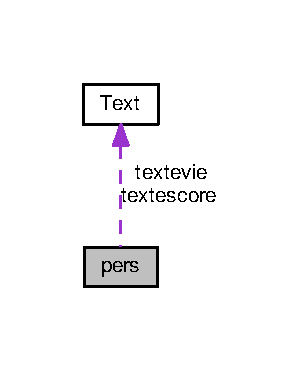
\includegraphics[width=144pt]{structpers__coll__graph}
\end{center}
\end{figure}
\subsection*{Data Fields}
\begin{DoxyCompactItemize}
\item 
S\+D\+L\+\_\+\+Surface $\ast$ {\bfseries bas}\hypertarget{structpers_a97425217365ebe97b60a7ff709293889}{}\label{structpers_a97425217365ebe97b60a7ff709293889}

\item 
S\+D\+L\+\_\+\+Surface $\ast$ {\bfseries haut}\hypertarget{structpers_a52c3a89d5f626dd8d7855b923dd74a98}{}\label{structpers_a52c3a89d5f626dd8d7855b923dd74a98}

\item 
S\+D\+L\+\_\+\+Surface $\ast$ {\bfseries gauche} \mbox{[}8\mbox{]}\hypertarget{structpers_a1e7eb13938d69dfdcd18c6ce8e3e8fc1}{}\label{structpers_a1e7eb13938d69dfdcd18c6ce8e3e8fc1}

\item 
S\+D\+L\+\_\+\+Surface $\ast$ {\bfseries droite} \mbox{[}8\mbox{]}\hypertarget{structpers_a41feac12596e95f916b0aeda8afaf9b1}{}\label{structpers_a41feac12596e95f916b0aeda8afaf9b1}

\item 
S\+D\+L\+\_\+\+Surface $\ast$ {\bfseries depart}\hypertarget{structpers_adcca1e384ac22f92d55ce6ed582845bf}{}\label{structpers_adcca1e384ac22f92d55ce6ed582845bf}

\item 
int {\bfseries left}\hypertarget{structpers_a5f64769124dbdb0dd030e59d60f19d69}{}\label{structpers_a5f64769124dbdb0dd030e59d60f19d69}

\item 
int {\bfseries right}\hypertarget{structpers_aad0039e0a768051bd52a83066c70fbf0}{}\label{structpers_aad0039e0a768051bd52a83066c70fbf0}

\item 
S\+D\+L\+\_\+\+Rect {\bfseries position\+\_\+joueur}\hypertarget{structpers_a7df8ffc6c20cd56d47109e7cfe56b846}{}\label{structpers_a7df8ffc6c20cd56d47109e7cfe56b846}

\item 
int {\bfseries score}\hypertarget{structpers_a6d7e4808902bf88fe8ad1cad683328c7}{}\label{structpers_a6d7e4808902bf88fe8ad1cad683328c7}

\item 
int {\bfseries vie}\hypertarget{structpers_ac0d08da120588d9771ad816ba6255c0a}{}\label{structpers_ac0d08da120588d9771ad816ba6255c0a}

\item 
\hyperlink{structText}{Text} {\bfseries textevie}\hypertarget{structpers_af0dc51b3c2878d4180413bf3980143da}{}\label{structpers_af0dc51b3c2878d4180413bf3980143da}

\item 
\hyperlink{structText}{Text} {\bfseries textescore}\hypertarget{structpers_a17e33c00db561982dba7c03351deedc1}{}\label{structpers_a17e33c00db561982dba7c03351deedc1}

\end{DoxyCompactItemize}


\subsection{Detailed Description}
struct for personnage 

The documentation for this struct was generated from the following file\+:\begin{DoxyCompactItemize}
\item 
pers.\+h\end{DoxyCompactItemize}

\hypertarget{structText}{}\section{Text Struct Reference}
\label{structText}\index{Text@{Text}}


struct for \hyperlink{structText}{Text}  




{\ttfamily \#include $<$utilitaire.\+h$>$}

\subsection*{Data Fields}
\begin{DoxyCompactItemize}
\item 
S\+D\+L\+\_\+\+Surface $\ast$ {\bfseries text\+Surface}\hypertarget{structText_aa62d89be189c1522d97c221b3c1fea81}{}\label{structText_aa62d89be189c1522d97c221b3c1fea81}

\item 
S\+D\+L\+\_\+\+Rect {\bfseries position\+Text}\hypertarget{structText_ad9efd8ca20e485d7c15790e748429345}{}\label{structText_ad9efd8ca20e485d7c15790e748429345}

\item 
char {\bfseries txt} \mbox{[}20\mbox{]}\hypertarget{structText_ae4c1e2eef4f3f19d5be9793e6e2df17b}{}\label{structText_ae4c1e2eef4f3f19d5be9793e6e2df17b}

\item 
S\+D\+L\+\_\+\+Color {\bfseries couleur\+Txt}\hypertarget{structText_a2b4f89e854de412a5d2e21ad5a827aa3}{}\label{structText_a2b4f89e854de412a5d2e21ad5a827aa3}

\item 
T\+T\+F\+\_\+\+Font $\ast$ {\bfseries police}\hypertarget{structText_a68484d7ee9aa7d5b600aa58245f143a5}{}\label{structText_a68484d7ee9aa7d5b600aa58245f143a5}

\end{DoxyCompactItemize}


\subsection{Detailed Description}
struct for \hyperlink{structText}{Text} 

The documentation for this struct was generated from the following file\+:\begin{DoxyCompactItemize}
\item 
utilitaire.\+h\end{DoxyCompactItemize}

\hypertarget{structTime}{}\section{Time Struct Reference}
\label{structTime}\index{Time@{Time}}


struct for time  




{\ttfamily \#include $<$utilitaire.\+h$>$}



Collaboration diagram for Time\+:
\nopagebreak
\begin{figure}[H]
\begin{center}
\leavevmode
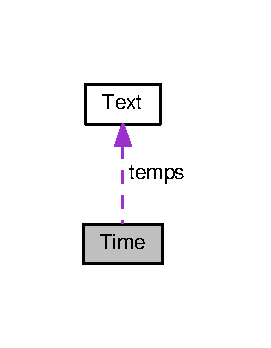
\includegraphics[width=130pt]{structTime__coll__graph}
\end{center}
\end{figure}
\subsection*{Data Fields}
\begin{DoxyCompactItemize}
\item 
int {\bfseries tempsdebut}\hypertarget{structTime_a6f3ddd3b01a77b15633b492e6a07664e}{}\label{structTime_a6f3ddd3b01a77b15633b492e6a07664e}

\item 
int {\bfseries mm}\hypertarget{structTime_add7853e0a8e3746cbfc85fe7ba73e00d}{}\label{structTime_add7853e0a8e3746cbfc85fe7ba73e00d}

\item 
int {\bfseries ss}\hypertarget{structTime_a98bc47508851fde020119b90e95784dc}{}\label{structTime_a98bc47508851fde020119b90e95784dc}

\item 
\hyperlink{structText}{Text} {\bfseries temps}\hypertarget{structTime_a5156d0ff2d9afb53bba51b4299402a75}{}\label{structTime_a5156d0ff2d9afb53bba51b4299402a75}

\end{DoxyCompactItemize}


\subsection{Detailed Description}
struct for time 

The documentation for this struct was generated from the following file\+:\begin{DoxyCompactItemize}
\item 
utilitaire.\+h\end{DoxyCompactItemize}

\chapter{File Documentation}
\hypertarget{main_8c}{}\section{main.\+c File Reference}
\label{main_8c}\index{main.\+c@{main.\+c}}


Testing Program.  


{\ttfamily \#include $<$stdio.\+h$>$}\\*
{\ttfamily \#include $<$stdlib.\+h$>$}\\*
{\ttfamily \#include $<$S\+D\+L/\+S\+D\+L.\+h$>$}\\*
{\ttfamily \#include $<$S\+D\+L/\+S\+D\+L\+\_\+image.\+h$>$}\\*
{\ttfamily \#include $<$S\+D\+L/\+S\+D\+L\+\_\+mixer.\+h$>$}\\*
{\ttfamily \#include $<$S\+D\+L/\+S\+D\+L\+\_\+ttf.\+h$>$}\\*
{\ttfamily \#include \char`\"{}pers.\+h\char`\"{}}\\*
Include dependency graph for main.\+c\+:\nopagebreak
\begin{figure}[H]
\begin{center}
\leavevmode
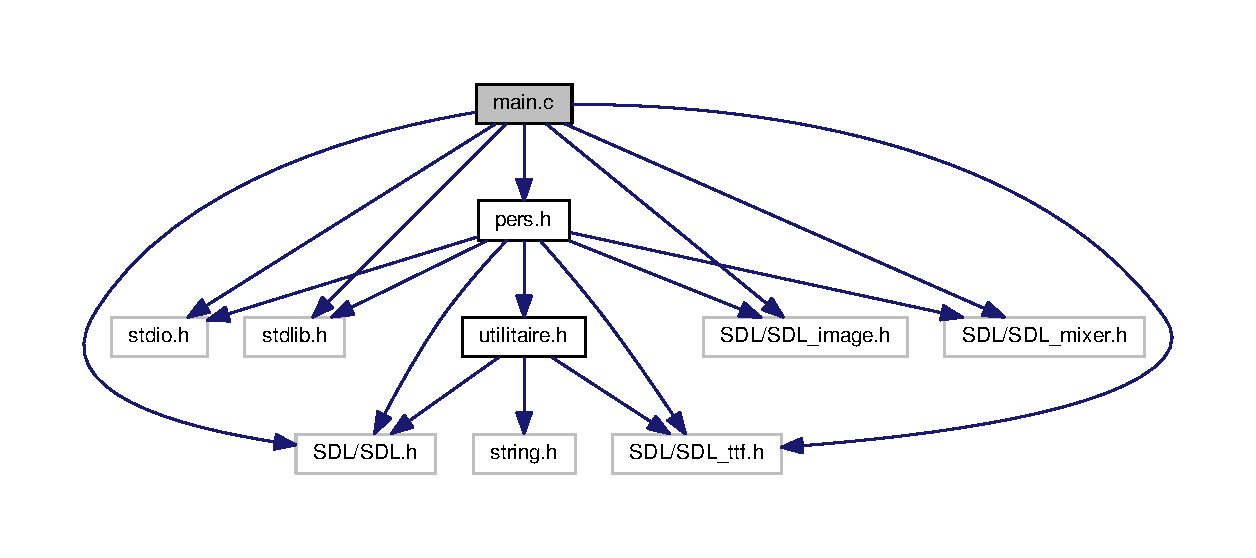
\includegraphics[width=350pt]{main_8c__incl}
\end{center}
\end{figure}
\subsection*{Functions}
\begin{DoxyCompactItemize}
\item 
int {\bfseries main} ()\hypertarget{main_8c_ae66f6b31b5ad750f1fe042a706a4e3d4}{}\label{main_8c_ae66f6b31b5ad750f1fe042a706a4e3d4}

\end{DoxyCompactItemize}


\subsection{Detailed Description}
Testing Program. 

\begin{DoxyAuthor}{Author}
C Team 
\end{DoxyAuthor}
\begin{DoxyVersion}{Version}
0.\+1 
\end{DoxyVersion}
\begin{DoxyDate}{Date}
Apr 01, 2020
\end{DoxyDate}
Testing program for gestion de vie et de score et de temps 
\hypertarget{pers_8c}{}\section{pers.\+c File Reference}
\label{pers_8c}\index{pers.\+c@{pers.\+c}}


Testing Program.  


{\ttfamily \#include \char`\"{}pers.\+h\char`\"{}}\\*
Include dependency graph for pers.\+c\+:\nopagebreak
\begin{figure}[H]
\begin{center}
\leavevmode
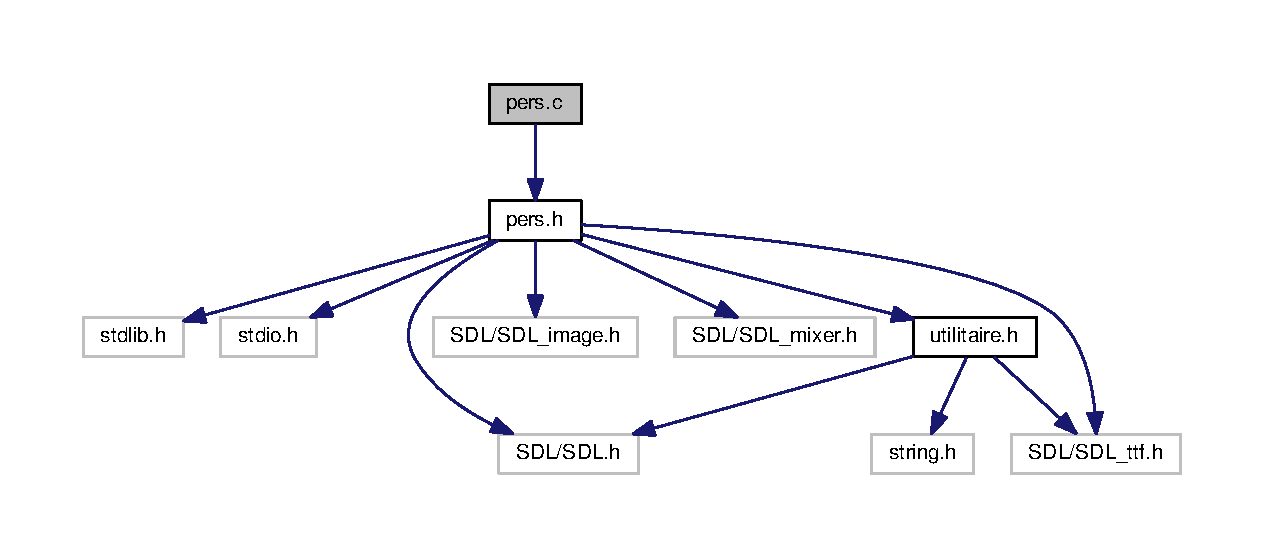
\includegraphics[width=350pt]{pers_8c__incl}
\end{center}
\end{figure}
\subsection*{Functions}
\begin{DoxyCompactItemize}
\item 
void \hyperlink{pers_8c_ac5ec830e2f41544edaf6caad25cca3fa}{initbackground} (\hyperlink{structimage}{image} $\ast$background)
\begin{DoxyCompactList}\small\item\em To initialize the background background . \end{DoxyCompactList}\item 
void \hyperlink{pers_8c_a5bdcb2a0ef37d39391dcb65810bca8d8}{initgameover} (\hyperlink{structimage}{image} $\ast$gameover)
\begin{DoxyCompactList}\small\item\em To initialize the image gameover . \end{DoxyCompactList}\item 
int \hyperlink{pers_8c_a9d18966b3d27827d37895d21d82b67e8}{initvie2} (\hyperlink{structText}{Text} $\ast$textevie, int $\ast$vie)
\begin{DoxyCompactList}\small\item\em To initialize the life . \end{DoxyCompactList}\item 
int \hyperlink{pers_8c_a85a9538b0b49ed9c18ae1f4b0b629c5c}{initscore2} (\hyperlink{structText}{Text} $\ast$textescore, int $\ast$score)
\begin{DoxyCompactList}\small\item\em To initialize the score . \end{DoxyCompactList}\item 
void \hyperlink{pers_8c_ae2c98fbc978d9bd667248e5c82709db3}{initperso2} (\hyperlink{structpers}{pers} $\ast$p)
\begin{DoxyCompactList}\small\item\em To initialize the pers p. \end{DoxyCompactList}\item 
int \hyperlink{pers_8c_a8e07134b10e7623c8a545ec6710d378b}{initvie1} (\hyperlink{structText}{Text} $\ast$textevie, int $\ast$vie)
\begin{DoxyCompactList}\small\item\em To initialize the life . \end{DoxyCompactList}\item 
int \hyperlink{pers_8c_a0d9c65d04ba25f85f85ef90893b268b8}{initscore1} (\hyperlink{structText}{Text} $\ast$textescore, int $\ast$score)
\begin{DoxyCompactList}\small\item\em To initialize the score . \end{DoxyCompactList}\item 
void \hyperlink{pers_8c_ab0270cd488d8e4d243920a717ea20a5d}{initperso1} (\hyperlink{structpers}{pers} $\ast$p)
\begin{DoxyCompactList}\small\item\em To initialize the pers p1. \end{DoxyCompactList}\item 
void \hyperlink{pers_8c_a80686d775976ea0644cb36e2f2aa3496}{initinput} (\hyperlink{structinput}{input} $\ast$in)
\begin{DoxyCompactList}\small\item\em To initialize the input . \end{DoxyCompactList}\item 
\hyperlink{structinput}{input} {\bfseries getinput} (int $\ast$done, \hyperlink{structinput}{input} in)\hypertarget{pers_8c_a7214aad146b64791f5b5861d448ef61a}{}\label{pers_8c_a7214aad146b64791f5b5861d448ef61a}

\item 
void \hyperlink{pers_8c_a561f27a91d81213da6a4525b19f15199}{updateperso1} (\hyperlink{structpers}{pers} $\ast$p, \hyperlink{structinput}{input} in, \hyperlink{structcollision}{collision} $\ast$col)
\begin{DoxyCompactList}\small\item\em To update the pers p1 . \end{DoxyCompactList}\item 
void \hyperlink{pers_8c_a3341f082d3873c90ca3ce2ec43f4be6a}{updateperso2} (\hyperlink{structpers}{pers} $\ast$p, \hyperlink{structinput}{input} in, \hyperlink{structcollision}{collision} $\ast$col)
\begin{DoxyCompactList}\small\item\em To update the pers p2 . \end{DoxyCompactList}\item 
void \hyperlink{pers_8c_ae21c24bbd1324afca4078aa3e159e7ea}{dipslayperso} (\hyperlink{structpers}{pers} p, S\+D\+L\+\_\+\+Surface $\ast$screen)
\begin{DoxyCompactList}\small\item\em To display the pers. \end{DoxyCompactList}\item 
void \hyperlink{pers_8c_a31a011d00a257a5b7747faf0f39214af}{displaybackground} (\hyperlink{structimage}{image} background, S\+D\+L\+\_\+\+Surface $\ast$screen)
\begin{DoxyCompactList}\small\item\em To display the background. \end{DoxyCompactList}\item 
void \hyperlink{pers_8c_af2a1df5255dbe633ffd06abc1f89a4b4}{displaygameover} (int $\ast$done, int vie, \hyperlink{structimage}{image} gameover, S\+D\+L\+\_\+\+Surface $\ast$screen)
\begin{DoxyCompactList}\small\item\em To display the gameover. \end{DoxyCompactList}\item 
void \hyperlink{pers_8c_abfeb5dfb3df9d00fe7cd9374e25fd52c}{freebackground} (\hyperlink{structimage}{image} background)
\begin{DoxyCompactList}\small\item\em To free background. \end{DoxyCompactList}\end{DoxyCompactItemize}


\subsection{Detailed Description}
Testing Program. 

\begin{DoxyAuthor}{Author}
C Team 
\end{DoxyAuthor}
\begin{DoxyVersion}{Version}
0.\+1 
\end{DoxyVersion}
\begin{DoxyDate}{Date}
Apr 01, 2020
\end{DoxyDate}
Testing pers 

\subsection{Function Documentation}
\index{pers.\+c@{pers.\+c}!dipslayperso@{dipslayperso}}
\index{dipslayperso@{dipslayperso}!pers.\+c@{pers.\+c}}
\subsubsection[{\texorpdfstring{dipslayperso(pers p, S\+D\+L\+\_\+\+Surface $\ast$screen)}{dipslayperso(pers p, SDL_Surface *screen)}}]{\setlength{\rightskip}{0pt plus 5cm}void dipslayperso (
\begin{DoxyParamCaption}
\item[{{\bf pers}}]{p, }
\item[{S\+D\+L\+\_\+\+Surface $\ast$}]{screen}
\end{DoxyParamCaption}
)}\hypertarget{pers_8c_ae21c24bbd1324afca4078aa3e159e7ea}{}\label{pers_8c_ae21c24bbd1324afca4078aa3e159e7ea}


To display the pers. 


\begin{DoxyParams}{Parameters}
{\em p} & the pers \\
\hline
{\em screen} & the screen \\
\hline
\end{DoxyParams}
\begin{DoxyReturn}{Returns}
nothing 
\end{DoxyReturn}


Here is the call graph for this function\+:\nopagebreak
\begin{figure}[H]
\begin{center}
\leavevmode
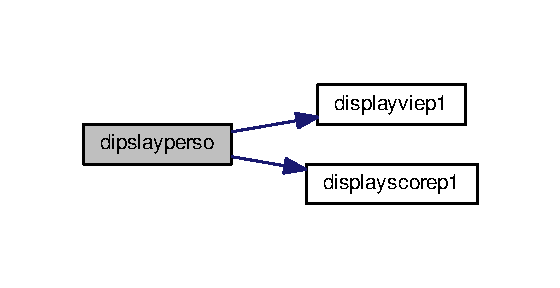
\includegraphics[width=269pt]{pers_8c_ae21c24bbd1324afca4078aa3e159e7ea_cgraph}
\end{center}
\end{figure}


\index{pers.\+c@{pers.\+c}!displaybackground@{displaybackground}}
\index{displaybackground@{displaybackground}!pers.\+c@{pers.\+c}}
\subsubsection[{\texorpdfstring{displaybackground(image background, S\+D\+L\+\_\+\+Surface $\ast$screen)}{displaybackground(image background, SDL_Surface *screen)}}]{\setlength{\rightskip}{0pt plus 5cm}void displaybackground (
\begin{DoxyParamCaption}
\item[{{\bf image}}]{background, }
\item[{S\+D\+L\+\_\+\+Surface $\ast$}]{screen}
\end{DoxyParamCaption}
)}\hypertarget{pers_8c_a31a011d00a257a5b7747faf0f39214af}{}\label{pers_8c_a31a011d00a257a5b7747faf0f39214af}


To display the background. 


\begin{DoxyParams}{Parameters}
{\em background} & the background \\
\hline
{\em screen} & the screen \\
\hline
\end{DoxyParams}
\begin{DoxyReturn}{Returns}
nothing 
\end{DoxyReturn}
\index{pers.\+c@{pers.\+c}!displaygameover@{displaygameover}}
\index{displaygameover@{displaygameover}!pers.\+c@{pers.\+c}}
\subsubsection[{\texorpdfstring{displaygameover(int $\ast$done, int vie, image gameover, S\+D\+L\+\_\+\+Surface $\ast$screen)}{displaygameover(int *done, int vie, image gameover, SDL_Surface *screen)}}]{\setlength{\rightskip}{0pt plus 5cm}void displaygameover (
\begin{DoxyParamCaption}
\item[{int $\ast$}]{done, }
\item[{int}]{vie, }
\item[{{\bf image}}]{gameover, }
\item[{S\+D\+L\+\_\+\+Surface $\ast$}]{screen}
\end{DoxyParamCaption}
)}\hypertarget{pers_8c_af2a1df5255dbe633ffd06abc1f89a4b4}{}\label{pers_8c_af2a1df5255dbe633ffd06abc1f89a4b4}


To display the gameover. 


\begin{DoxyParams}{Parameters}
{\em gameover} & the image of gameover \\
\hline
{\em screen} & the screen \\
\hline
{\em vie} & the number of life \\
\hline
\end{DoxyParams}
\begin{DoxyReturn}{Returns}
nothing 
\end{DoxyReturn}
\index{pers.\+c@{pers.\+c}!freebackground@{freebackground}}
\index{freebackground@{freebackground}!pers.\+c@{pers.\+c}}
\subsubsection[{\texorpdfstring{freebackground(image background)}{freebackground(image background)}}]{\setlength{\rightskip}{0pt plus 5cm}void freebackground (
\begin{DoxyParamCaption}
\item[{{\bf image}}]{background}
\end{DoxyParamCaption}
)}\hypertarget{pers_8c_abfeb5dfb3df9d00fe7cd9374e25fd52c}{}\label{pers_8c_abfeb5dfb3df9d00fe7cd9374e25fd52c}


To free background. 


\begin{DoxyParams}{Parameters}
{\em background} & the background. \\
\hline
\end{DoxyParams}
\begin{DoxyReturn}{Returns}
Nothing 
\end{DoxyReturn}
\index{pers.\+c@{pers.\+c}!initbackground@{initbackground}}
\index{initbackground@{initbackground}!pers.\+c@{pers.\+c}}
\subsubsection[{\texorpdfstring{initbackground(image $\ast$background)}{initbackground(image *background)}}]{\setlength{\rightskip}{0pt plus 5cm}void initbackground (
\begin{DoxyParamCaption}
\item[{{\bf image} $\ast$}]{background}
\end{DoxyParamCaption}
)}\hypertarget{pers_8c_ac5ec830e2f41544edaf6caad25cca3fa}{}\label{pers_8c_ac5ec830e2f41544edaf6caad25cca3fa}


To initialize the background background . 


\begin{DoxyParams}{Parameters}
{\em background} & the background \\
\hline
\end{DoxyParams}
\begin{DoxyReturn}{Returns}
Nothing 
\end{DoxyReturn}
\index{pers.\+c@{pers.\+c}!initgameover@{initgameover}}
\index{initgameover@{initgameover}!pers.\+c@{pers.\+c}}
\subsubsection[{\texorpdfstring{initgameover(image $\ast$gameover)}{initgameover(image *gameover)}}]{\setlength{\rightskip}{0pt plus 5cm}void initgameover (
\begin{DoxyParamCaption}
\item[{{\bf image} $\ast$}]{gameover}
\end{DoxyParamCaption}
)}\hypertarget{pers_8c_a5bdcb2a0ef37d39391dcb65810bca8d8}{}\label{pers_8c_a5bdcb2a0ef37d39391dcb65810bca8d8}


To initialize the image gameover . 


\begin{DoxyParams}{Parameters}
{\em gameover} & the image \\
\hline
\end{DoxyParams}
\begin{DoxyReturn}{Returns}
Nothing 
\end{DoxyReturn}
\index{pers.\+c@{pers.\+c}!initinput@{initinput}}
\index{initinput@{initinput}!pers.\+c@{pers.\+c}}
\subsubsection[{\texorpdfstring{initinput(input $\ast$in)}{initinput(input *in)}}]{\setlength{\rightskip}{0pt plus 5cm}void initinput (
\begin{DoxyParamCaption}
\item[{{\bf input} $\ast$}]{in}
\end{DoxyParamCaption}
)}\hypertarget{pers_8c_a80686d775976ea0644cb36e2f2aa3496}{}\label{pers_8c_a80686d775976ea0644cb36e2f2aa3496}


To initialize the input . 


\begin{DoxyParams}{Parameters}
{\em in} & the input \\
\hline
\end{DoxyParams}
\begin{DoxyReturn}{Returns}
nothing 
\end{DoxyReturn}
\index{pers.\+c@{pers.\+c}!initperso1@{initperso1}}
\index{initperso1@{initperso1}!pers.\+c@{pers.\+c}}
\subsubsection[{\texorpdfstring{initperso1(pers $\ast$p)}{initperso1(pers *p)}}]{\setlength{\rightskip}{0pt plus 5cm}void initperso1 (
\begin{DoxyParamCaption}
\item[{{\bf pers} $\ast$}]{p}
\end{DoxyParamCaption}
)}\hypertarget{pers_8c_ab0270cd488d8e4d243920a717ea20a5d}{}\label{pers_8c_ab0270cd488d8e4d243920a717ea20a5d}


To initialize the pers p1. 


\begin{DoxyParams}{Parameters}
{\em p} & the pers \\
\hline
\end{DoxyParams}
\begin{DoxyReturn}{Returns}
nothing 
\end{DoxyReturn}


Here is the call graph for this function\+:\nopagebreak
\begin{figure}[H]
\begin{center}
\leavevmode
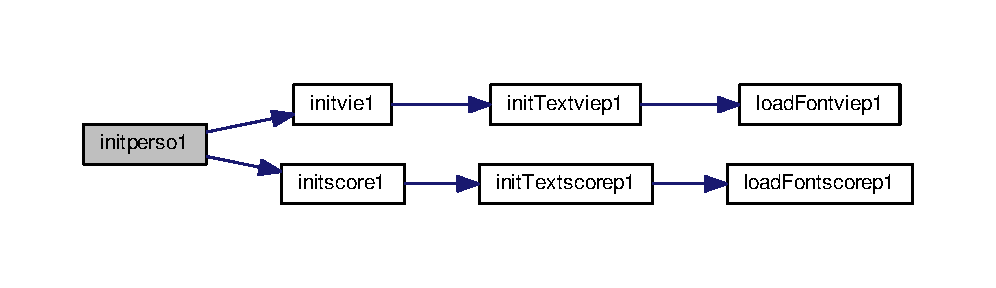
\includegraphics[width=350pt]{pers_8c_ab0270cd488d8e4d243920a717ea20a5d_cgraph}
\end{center}
\end{figure}


\index{pers.\+c@{pers.\+c}!initperso2@{initperso2}}
\index{initperso2@{initperso2}!pers.\+c@{pers.\+c}}
\subsubsection[{\texorpdfstring{initperso2(pers $\ast$p)}{initperso2(pers *p)}}]{\setlength{\rightskip}{0pt plus 5cm}void initperso2 (
\begin{DoxyParamCaption}
\item[{{\bf pers} $\ast$}]{p}
\end{DoxyParamCaption}
)}\hypertarget{pers_8c_ae2c98fbc978d9bd667248e5c82709db3}{}\label{pers_8c_ae2c98fbc978d9bd667248e5c82709db3}


To initialize the pers p. 


\begin{DoxyParams}{Parameters}
{\em p} & the pers \\
\hline
\end{DoxyParams}
\begin{DoxyReturn}{Returns}
nothing 
\end{DoxyReturn}


Here is the call graph for this function\+:\nopagebreak
\begin{figure}[H]
\begin{center}
\leavevmode
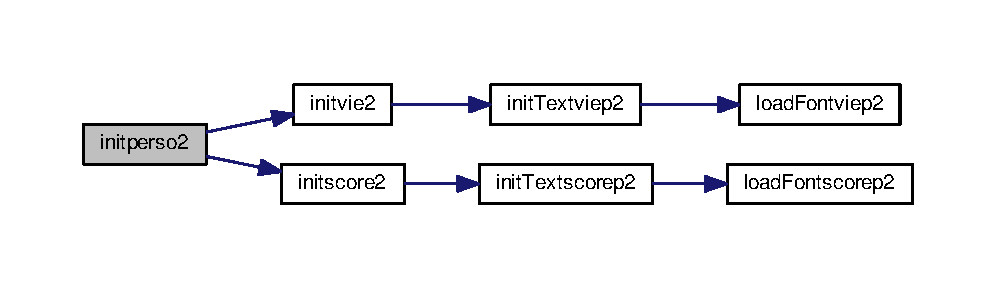
\includegraphics[width=350pt]{pers_8c_ae2c98fbc978d9bd667248e5c82709db3_cgraph}
\end{center}
\end{figure}


\index{pers.\+c@{pers.\+c}!initscore1@{initscore1}}
\index{initscore1@{initscore1}!pers.\+c@{pers.\+c}}
\subsubsection[{\texorpdfstring{initscore1(\+Text $\ast$textescore, int $\ast$score)}{initscore1(Text *textescore, int *score)}}]{\setlength{\rightskip}{0pt plus 5cm}int initscore1 (
\begin{DoxyParamCaption}
\item[{{\bf Text} $\ast$}]{textescore, }
\item[{int $\ast$}]{score}
\end{DoxyParamCaption}
)}\hypertarget{pers_8c_a0d9c65d04ba25f85f85ef90893b268b8}{}\label{pers_8c_a0d9c65d04ba25f85f85ef90893b268b8}


To initialize the score . 


\begin{DoxyParams}{Parameters}
{\em score} & the number of score \\
\hline
{\em textescore} & the text of score \\
\hline
\end{DoxyParams}
\begin{DoxyReturn}{Returns}
int 
\end{DoxyReturn}


Here is the call graph for this function\+:\nopagebreak
\begin{figure}[H]
\begin{center}
\leavevmode
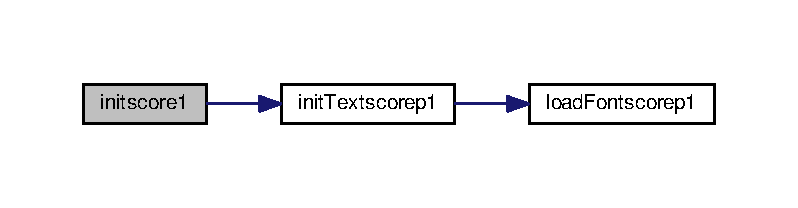
\includegraphics[width=350pt]{pers_8c_a0d9c65d04ba25f85f85ef90893b268b8_cgraph}
\end{center}
\end{figure}




Here is the caller graph for this function\+:\nopagebreak
\begin{figure}[H]
\begin{center}
\leavevmode
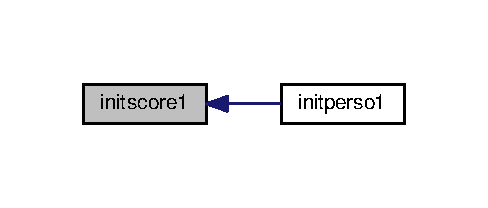
\includegraphics[width=234pt]{pers_8c_a0d9c65d04ba25f85f85ef90893b268b8_icgraph}
\end{center}
\end{figure}


\index{pers.\+c@{pers.\+c}!initscore2@{initscore2}}
\index{initscore2@{initscore2}!pers.\+c@{pers.\+c}}
\subsubsection[{\texorpdfstring{initscore2(\+Text $\ast$textescore, int $\ast$score)}{initscore2(Text *textescore, int *score)}}]{\setlength{\rightskip}{0pt plus 5cm}int initscore2 (
\begin{DoxyParamCaption}
\item[{{\bf Text} $\ast$}]{textescore, }
\item[{int $\ast$}]{score}
\end{DoxyParamCaption}
)}\hypertarget{pers_8c_a85a9538b0b49ed9c18ae1f4b0b629c5c}{}\label{pers_8c_a85a9538b0b49ed9c18ae1f4b0b629c5c}


To initialize the score . 


\begin{DoxyParams}{Parameters}
{\em score} & the number of score \\
\hline
{\em textescore} & the text of score \\
\hline
\end{DoxyParams}
\begin{DoxyReturn}{Returns}
int 
\end{DoxyReturn}


Here is the call graph for this function\+:\nopagebreak
\begin{figure}[H]
\begin{center}
\leavevmode
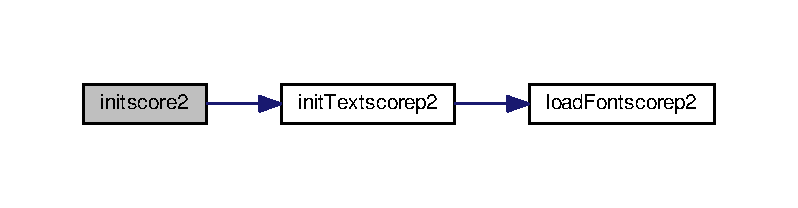
\includegraphics[width=350pt]{pers_8c_a85a9538b0b49ed9c18ae1f4b0b629c5c_cgraph}
\end{center}
\end{figure}




Here is the caller graph for this function\+:\nopagebreak
\begin{figure}[H]
\begin{center}
\leavevmode
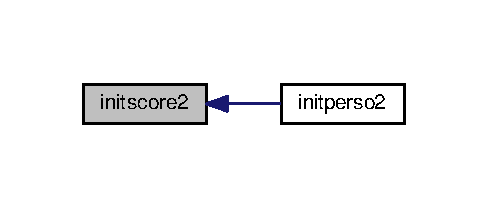
\includegraphics[width=234pt]{pers_8c_a85a9538b0b49ed9c18ae1f4b0b629c5c_icgraph}
\end{center}
\end{figure}


\index{pers.\+c@{pers.\+c}!initvie1@{initvie1}}
\index{initvie1@{initvie1}!pers.\+c@{pers.\+c}}
\subsubsection[{\texorpdfstring{initvie1(\+Text $\ast$textevie, int $\ast$vie)}{initvie1(Text *textevie, int *vie)}}]{\setlength{\rightskip}{0pt plus 5cm}int initvie1 (
\begin{DoxyParamCaption}
\item[{{\bf Text} $\ast$}]{textevie, }
\item[{int $\ast$}]{vie}
\end{DoxyParamCaption}
)}\hypertarget{pers_8c_a8e07134b10e7623c8a545ec6710d378b}{}\label{pers_8c_a8e07134b10e7623c8a545ec6710d378b}


To initialize the life . 


\begin{DoxyParams}{Parameters}
{\em vie} & the number of life \\
\hline
{\em textevie} & the text of life \\
\hline
\end{DoxyParams}
\begin{DoxyReturn}{Returns}
int 
\end{DoxyReturn}


Here is the call graph for this function\+:\nopagebreak
\begin{figure}[H]
\begin{center}
\leavevmode
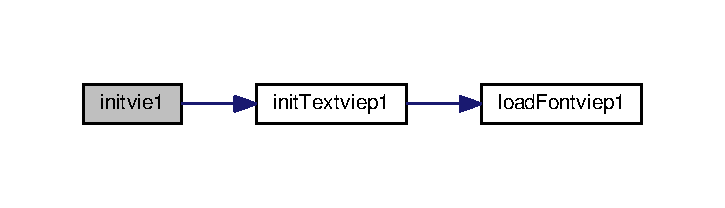
\includegraphics[width=348pt]{pers_8c_a8e07134b10e7623c8a545ec6710d378b_cgraph}
\end{center}
\end{figure}




Here is the caller graph for this function\+:\nopagebreak
\begin{figure}[H]
\begin{center}
\leavevmode
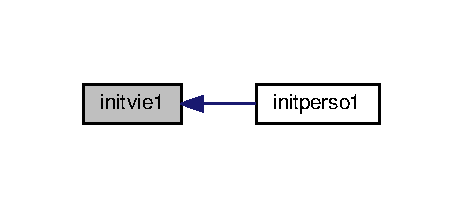
\includegraphics[width=222pt]{pers_8c_a8e07134b10e7623c8a545ec6710d378b_icgraph}
\end{center}
\end{figure}


\index{pers.\+c@{pers.\+c}!initvie2@{initvie2}}
\index{initvie2@{initvie2}!pers.\+c@{pers.\+c}}
\subsubsection[{\texorpdfstring{initvie2(\+Text $\ast$textevie, int $\ast$vie)}{initvie2(Text *textevie, int *vie)}}]{\setlength{\rightskip}{0pt plus 5cm}int initvie2 (
\begin{DoxyParamCaption}
\item[{{\bf Text} $\ast$}]{textevie, }
\item[{int $\ast$}]{vie}
\end{DoxyParamCaption}
)}\hypertarget{pers_8c_a9d18966b3d27827d37895d21d82b67e8}{}\label{pers_8c_a9d18966b3d27827d37895d21d82b67e8}


To initialize the life . 


\begin{DoxyParams}{Parameters}
{\em vie} & the number of life \\
\hline
{\em textevie} & the text of life \\
\hline
\end{DoxyParams}
\begin{DoxyReturn}{Returns}
int 
\end{DoxyReturn}


Here is the call graph for this function\+:\nopagebreak
\begin{figure}[H]
\begin{center}
\leavevmode
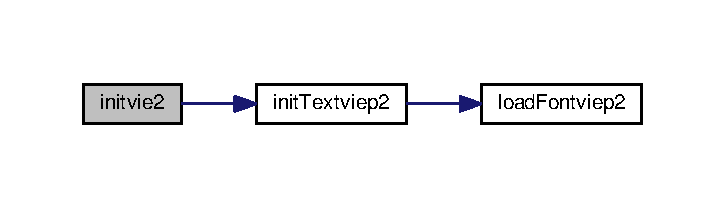
\includegraphics[width=348pt]{pers_8c_a9d18966b3d27827d37895d21d82b67e8_cgraph}
\end{center}
\end{figure}




Here is the caller graph for this function\+:\nopagebreak
\begin{figure}[H]
\begin{center}
\leavevmode
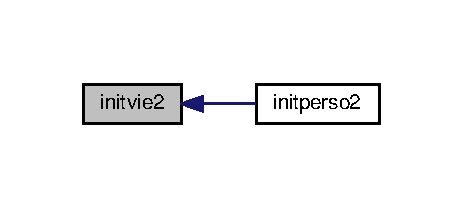
\includegraphics[width=222pt]{pers_8c_a9d18966b3d27827d37895d21d82b67e8_icgraph}
\end{center}
\end{figure}


\index{pers.\+c@{pers.\+c}!updateperso1@{updateperso1}}
\index{updateperso1@{updateperso1}!pers.\+c@{pers.\+c}}
\subsubsection[{\texorpdfstring{updateperso1(pers $\ast$p, input in, collision $\ast$col)}{updateperso1(pers *p, input in, collision *col)}}]{\setlength{\rightskip}{0pt plus 5cm}void updateperso1 (
\begin{DoxyParamCaption}
\item[{{\bf pers} $\ast$}]{p, }
\item[{{\bf input}}]{in, }
\item[{{\bf collision} $\ast$}]{col}
\end{DoxyParamCaption}
)}\hypertarget{pers_8c_a561f27a91d81213da6a4525b19f15199}{}\label{pers_8c_a561f27a91d81213da6a4525b19f15199}


To update the pers p1 . 


\begin{DoxyParams}{Parameters}
{\em p} & the pers \\
\hline
{\em in} & the input \\
\hline
{\em col} & the collision \\
\hline
\end{DoxyParams}
\begin{DoxyReturn}{Returns}
nothing 
\end{DoxyReturn}


Here is the call graph for this function\+:\nopagebreak
\begin{figure}[H]
\begin{center}
\leavevmode
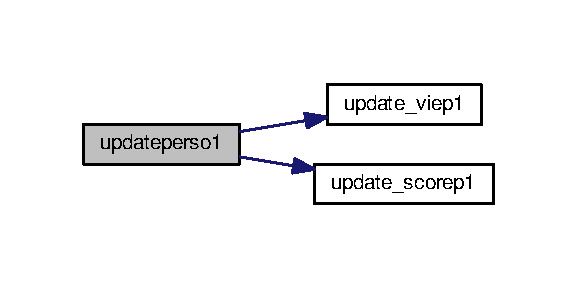
\includegraphics[width=277pt]{pers_8c_a561f27a91d81213da6a4525b19f15199_cgraph}
\end{center}
\end{figure}


\index{pers.\+c@{pers.\+c}!updateperso2@{updateperso2}}
\index{updateperso2@{updateperso2}!pers.\+c@{pers.\+c}}
\subsubsection[{\texorpdfstring{updateperso2(pers $\ast$p, input in, collision $\ast$col)}{updateperso2(pers *p, input in, collision *col)}}]{\setlength{\rightskip}{0pt plus 5cm}void updateperso2 (
\begin{DoxyParamCaption}
\item[{{\bf pers} $\ast$}]{p, }
\item[{{\bf input}}]{in, }
\item[{{\bf collision} $\ast$}]{col}
\end{DoxyParamCaption}
)}\hypertarget{pers_8c_a3341f082d3873c90ca3ce2ec43f4be6a}{}\label{pers_8c_a3341f082d3873c90ca3ce2ec43f4be6a}


To update the pers p2 . 


\begin{DoxyParams}{Parameters}
{\em p} & the pers \\
\hline
{\em in} & the input \\
\hline
{\em col} & the collision \\
\hline
\end{DoxyParams}
\begin{DoxyReturn}{Returns}
nothing 
\end{DoxyReturn}


Here is the call graph for this function\+:\nopagebreak
\begin{figure}[H]
\begin{center}
\leavevmode
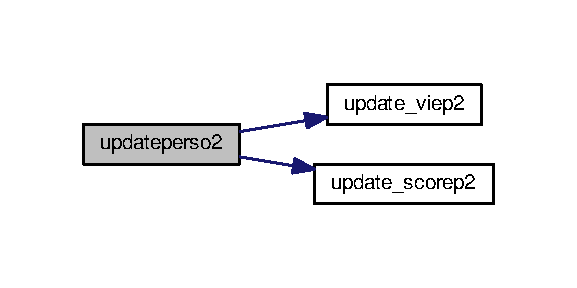
\includegraphics[width=277pt]{pers_8c_a3341f082d3873c90ca3ce2ec43f4be6a_cgraph}
\end{center}
\end{figure}



\hypertarget{utilitaire_8c}{}\section{utilitaire.\+c File Reference}
\label{utilitaire_8c}\index{utilitaire.\+c@{utilitaire.\+c}}
{\ttfamily \#include $<$stdio.\+h$>$}\\*
{\ttfamily \#include $<$stdlib.\+h$>$}\\*
{\ttfamily \#include $<$S\+D\+L/\+S\+D\+L\+\_\+image.\+h$>$}\\*
{\ttfamily \#include $<$S\+D\+L/\+S\+D\+L\+\_\+ttf.\+h$>$}\\*
{\ttfamily \#include \char`\"{}utilitaire.\+h\char`\"{}}\\*
Include dependency graph for utilitaire.\+c\+:\nopagebreak
\begin{figure}[H]
\begin{center}
\leavevmode
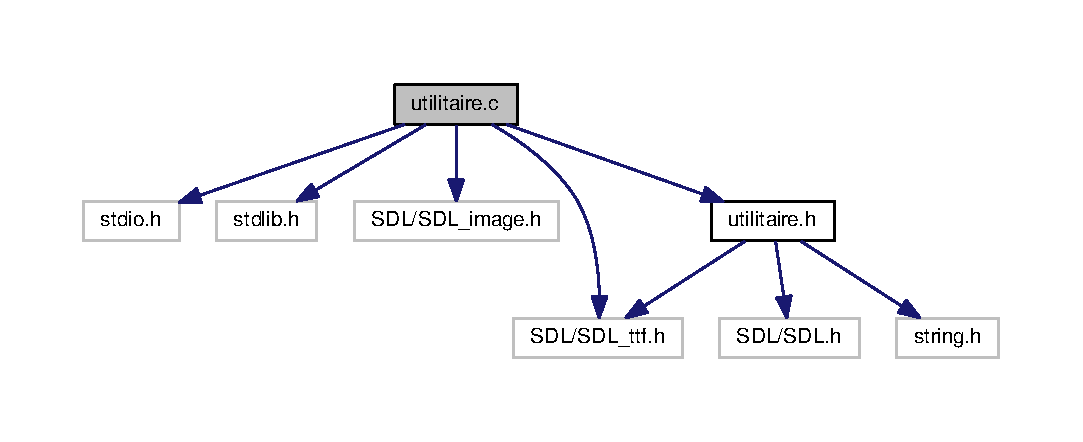
\includegraphics[width=350pt]{utilitaire_8c__incl}
\end{center}
\end{figure}
\subsection*{Functions}
\begin{DoxyCompactItemize}
\item 
int \hyperlink{utilitaire_8c_a9f0f8886c9c3e6e8469cb1a24a8c9ed6}{init\+Textviep1} (\hyperlink{structText}{Text} $\ast$T)
\begin{DoxyCompactList}\small\item\em To initialize the text T . \end{DoxyCompactList}\item 
int \hyperlink{utilitaire_8c_aa94706beac591b2437d6e27e8b1a6551}{load\+Fontviep1} (\hyperlink{structText}{Text} $\ast$T, char $\ast$path)
\begin{DoxyCompactList}\small\item\em To load the font T . \end{DoxyCompactList}\item 
void \hyperlink{utilitaire_8c_a8876655d6513fd06f7c4a3d07f7d92e3}{update\+\_\+viep1} (\hyperlink{structText}{Text} $\ast$T, int $\ast$vies, \hyperlink{structcollision}{collision} col)
\begin{DoxyCompactList}\small\item\em To update vie . \end{DoxyCompactList}\item 
void \hyperlink{utilitaire_8c_a773161d7c59e95006ab9da2b216c0db3}{displayviep1} (\hyperlink{structText}{Text} T, S\+D\+L\+\_\+\+Surface $\ast$screen)
\begin{DoxyCompactList}\small\item\em To display life . \end{DoxyCompactList}\item 
void \hyperlink{utilitaire_8c_a865dc044acaf6977b1104b40d1ca9971}{free\+Textviep1} (\hyperlink{structText}{Text} T)
\begin{DoxyCompactList}\small\item\em To free text vie . \end{DoxyCompactList}\item 
int \hyperlink{utilitaire_8c_ad140cfd864e9a32a4209627b2c4388dd}{init\+Textviep2} (\hyperlink{structText}{Text} $\ast$T)
\begin{DoxyCompactList}\small\item\em To initialize the text T . \end{DoxyCompactList}\item 
int \hyperlink{utilitaire_8c_a14b318435a12ec6e651f120e034993fe}{load\+Fontviep2} (\hyperlink{structText}{Text} $\ast$T, char $\ast$path)
\begin{DoxyCompactList}\small\item\em To load the font T . \end{DoxyCompactList}\item 
void \hyperlink{utilitaire_8c_a9601e16efa9686e1f560ef5a4a4727bf}{update\+\_\+viep2} (\hyperlink{structText}{Text} $\ast$T, int $\ast$vies, \hyperlink{structcollision}{collision} col)
\begin{DoxyCompactList}\small\item\em To update vie . \end{DoxyCompactList}\item 
void \hyperlink{utilitaire_8c_aefc12fb9d73f6f06d60d1e764a1e12db}{displayviep2} (\hyperlink{structText}{Text} T, S\+D\+L\+\_\+\+Surface $\ast$screen)
\begin{DoxyCompactList}\small\item\em To display life . \end{DoxyCompactList}\item 
void \hyperlink{utilitaire_8c_a03165062187b615ea2c14322e49bac5d}{free\+Textviep2} (\hyperlink{structText}{Text} T)
\begin{DoxyCompactList}\small\item\em To free text vie . \end{DoxyCompactList}\item 
void \hyperlink{utilitaire_8c_a5929c26a66049460dc58b8c92a6d0b2f}{Timer} (int $\ast$tempsdebut)
\begin{DoxyCompactList}\small\item\em To count \hyperlink{structTime}{Time} . \end{DoxyCompactList}\item 
void \hyperlink{utilitaire_8c_a2bbd14a997f1fa7fd246f24ead3b50f8}{inittemps} (\hyperlink{structTime}{Time} $\ast$t)
\begin{DoxyCompactList}\small\item\em To initialize the time . \end{DoxyCompactList}\item 
int \hyperlink{utilitaire_8c_ae326325c6cbb8e991873fc3da6a8265e}{init\+Texttime} (\hyperlink{structText}{Text} $\ast$T)
\begin{DoxyCompactList}\small\item\em To initialize the text T . \end{DoxyCompactList}\item 
int \hyperlink{utilitaire_8c_abf80670169d96288d8a4b673ad90a80a}{load\+Fonttime} (\hyperlink{structText}{Text} $\ast$T, char $\ast$path)
\begin{DoxyCompactList}\small\item\em To load the font T . \end{DoxyCompactList}\item 
void \hyperlink{utilitaire_8c_abc558b87e2e48a9f354536407ee6abbd}{update\+\_\+time} (\hyperlink{structTime}{Time} $\ast$T)
\begin{DoxyCompactList}\small\item\em To update time . \end{DoxyCompactList}\item 
void \hyperlink{utilitaire_8c_aeaf577c70c6195dd63b6424c46025020}{displaytime} (\hyperlink{structTime}{Time} T, S\+D\+L\+\_\+\+Surface $\ast$screen)
\begin{DoxyCompactList}\small\item\em To display time . \end{DoxyCompactList}\item 
void \hyperlink{utilitaire_8c_a1aea230c66513887e2a8dba8b3d2d075}{free\+Texttime} (\hyperlink{structText}{Text} T)
\begin{DoxyCompactList}\small\item\em To free text time . \end{DoxyCompactList}\item 
int \hyperlink{utilitaire_8c_a55245cb1f67d5bd884e547b37bd4d1b3}{init\+Textscorep1} (\hyperlink{structText}{Text} $\ast$T)
\begin{DoxyCompactList}\small\item\em To initialize the text T . \end{DoxyCompactList}\item 
int \hyperlink{utilitaire_8c_a51c7c5c649ffa053546af592ad26fe9b}{load\+Fontscorep1} (\hyperlink{structText}{Text} $\ast$T, char $\ast$path)
\begin{DoxyCompactList}\small\item\em To load the font T . \end{DoxyCompactList}\item 
void \hyperlink{utilitaire_8c_a43d377ba6c658485c2058b8c4feafc45}{update\+\_\+scorep1} (\hyperlink{structText}{Text} $\ast$T, int $\ast$score, \hyperlink{structcollision}{collision} col)
\begin{DoxyCompactList}\small\item\em To update score . \end{DoxyCompactList}\item 
void \hyperlink{utilitaire_8c_a82eb1d475b86a63e03adccb3220d901a}{displayscorep1} (\hyperlink{structText}{Text} T, S\+D\+L\+\_\+\+Surface $\ast$screen)
\begin{DoxyCompactList}\small\item\em To display score . \end{DoxyCompactList}\item 
void \hyperlink{utilitaire_8c_a54559142e76216168931e021ff6e4c11}{free\+Textscorep1} (\hyperlink{structText}{Text} T)
\begin{DoxyCompactList}\small\item\em To free text score. \end{DoxyCompactList}\item 
int \hyperlink{utilitaire_8c_a45b667d61b2ed92906aa25efcba9c5a3}{init\+Textscorep2} (\hyperlink{structText}{Text} $\ast$T)
\begin{DoxyCompactList}\small\item\em To initialize the text T . \end{DoxyCompactList}\item 
int \hyperlink{utilitaire_8c_a47f18f3dfebbf72ac94e1ab431f2212b}{load\+Fontscorep2} (\hyperlink{structText}{Text} $\ast$T, char $\ast$path)
\begin{DoxyCompactList}\small\item\em To load the font T . \end{DoxyCompactList}\item 
void \hyperlink{utilitaire_8c_ad8da31bfa2e50fc4e771bfad1d769c95}{update\+\_\+scorep2} (\hyperlink{structText}{Text} $\ast$T, int $\ast$score, \hyperlink{structcollision}{collision} col)
\begin{DoxyCompactList}\small\item\em To update score . \end{DoxyCompactList}\item 
void \hyperlink{utilitaire_8c_a885861529ca9ba36299b69d3fa6f3076}{displayscorep2} (\hyperlink{structText}{Text} T, S\+D\+L\+\_\+\+Surface $\ast$screen)
\begin{DoxyCompactList}\small\item\em To display score . \end{DoxyCompactList}\item 
void \hyperlink{utilitaire_8c_a5321d82b1f101582a7fceef97065b9c6}{free\+Textscorep2} (\hyperlink{structText}{Text} T)
\begin{DoxyCompactList}\small\item\em To free text score. \end{DoxyCompactList}\end{DoxyCompactItemize}


\subsection{Function Documentation}
\index{utilitaire.\+c@{utilitaire.\+c}!displayscorep1@{displayscorep1}}
\index{displayscorep1@{displayscorep1}!utilitaire.\+c@{utilitaire.\+c}}
\subsubsection[{\texorpdfstring{displayscorep1(\+Text T, S\+D\+L\+\_\+\+Surface $\ast$screen)}{displayscorep1(Text T, SDL_Surface *screen)}}]{\setlength{\rightskip}{0pt plus 5cm}void displayscorep1 (
\begin{DoxyParamCaption}
\item[{{\bf Text}}]{T, }
\item[{S\+D\+L\+\_\+\+Surface $\ast$}]{screen}
\end{DoxyParamCaption}
)}\hypertarget{utilitaire_8c_a82eb1d475b86a63e03adccb3220d901a}{}\label{utilitaire_8c_a82eb1d475b86a63e03adccb3220d901a}


To display score . 


\begin{DoxyParams}{Parameters}
{\em T} & the text of score. \\
\hline
{\em screen} & . \\
\hline
\end{DoxyParams}
\begin{DoxyReturn}{Returns}
Nothing 
\end{DoxyReturn}


Here is the caller graph for this function\+:\nopagebreak
\begin{figure}[H]
\begin{center}
\leavevmode
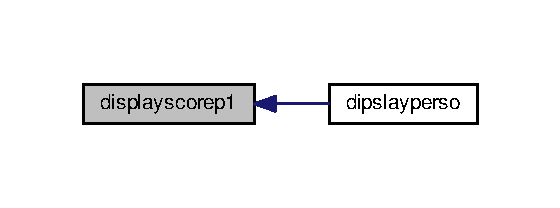
\includegraphics[width=269pt]{utilitaire_8c_a82eb1d475b86a63e03adccb3220d901a_icgraph}
\end{center}
\end{figure}


\index{utilitaire.\+c@{utilitaire.\+c}!displayscorep2@{displayscorep2}}
\index{displayscorep2@{displayscorep2}!utilitaire.\+c@{utilitaire.\+c}}
\subsubsection[{\texorpdfstring{displayscorep2(\+Text T, S\+D\+L\+\_\+\+Surface $\ast$screen)}{displayscorep2(Text T, SDL_Surface *screen)}}]{\setlength{\rightskip}{0pt plus 5cm}void displayscorep2 (
\begin{DoxyParamCaption}
\item[{{\bf Text}}]{T, }
\item[{S\+D\+L\+\_\+\+Surface $\ast$}]{screen}
\end{DoxyParamCaption}
)}\hypertarget{utilitaire_8c_a885861529ca9ba36299b69d3fa6f3076}{}\label{utilitaire_8c_a885861529ca9ba36299b69d3fa6f3076}


To display score . 


\begin{DoxyParams}{Parameters}
{\em T} & the text of score. \\
\hline
{\em screen} & . \\
\hline
\end{DoxyParams}
\begin{DoxyReturn}{Returns}
Nothing 
\end{DoxyReturn}
\index{utilitaire.\+c@{utilitaire.\+c}!displaytime@{displaytime}}
\index{displaytime@{displaytime}!utilitaire.\+c@{utilitaire.\+c}}
\subsubsection[{\texorpdfstring{displaytime(\+Time T, S\+D\+L\+\_\+\+Surface $\ast$screen)}{displaytime(Time T, SDL_Surface *screen)}}]{\setlength{\rightskip}{0pt plus 5cm}void displaytime (
\begin{DoxyParamCaption}
\item[{{\bf Time}}]{T, }
\item[{S\+D\+L\+\_\+\+Surface $\ast$}]{screen}
\end{DoxyParamCaption}
)}\hypertarget{utilitaire_8c_aeaf577c70c6195dd63b6424c46025020}{}\label{utilitaire_8c_aeaf577c70c6195dd63b6424c46025020}


To display time . 


\begin{DoxyParams}{Parameters}
{\em T} & the text of time. \\
\hline
{\em screen} & . \\
\hline
\end{DoxyParams}
\begin{DoxyReturn}{Returns}
Nothing 
\end{DoxyReturn}
\index{utilitaire.\+c@{utilitaire.\+c}!displayviep1@{displayviep1}}
\index{displayviep1@{displayviep1}!utilitaire.\+c@{utilitaire.\+c}}
\subsubsection[{\texorpdfstring{displayviep1(\+Text T, S\+D\+L\+\_\+\+Surface $\ast$screen)}{displayviep1(Text T, SDL_Surface *screen)}}]{\setlength{\rightskip}{0pt plus 5cm}void displayviep1 (
\begin{DoxyParamCaption}
\item[{{\bf Text}}]{T, }
\item[{S\+D\+L\+\_\+\+Surface $\ast$}]{screen}
\end{DoxyParamCaption}
)}\hypertarget{utilitaire_8c_a773161d7c59e95006ab9da2b216c0db3}{}\label{utilitaire_8c_a773161d7c59e95006ab9da2b216c0db3}


To display life . 


\begin{DoxyParams}{Parameters}
{\em T} & the text of vie. \\
\hline
{\em screen} & . \\
\hline
\end{DoxyParams}
\begin{DoxyReturn}{Returns}
Nothing 
\end{DoxyReturn}


Here is the caller graph for this function\+:\nopagebreak
\begin{figure}[H]
\begin{center}
\leavevmode
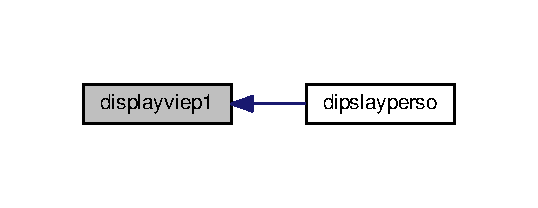
\includegraphics[width=258pt]{utilitaire_8c_a773161d7c59e95006ab9da2b216c0db3_icgraph}
\end{center}
\end{figure}


\index{utilitaire.\+c@{utilitaire.\+c}!displayviep2@{displayviep2}}
\index{displayviep2@{displayviep2}!utilitaire.\+c@{utilitaire.\+c}}
\subsubsection[{\texorpdfstring{displayviep2(\+Text T, S\+D\+L\+\_\+\+Surface $\ast$screen)}{displayviep2(Text T, SDL_Surface *screen)}}]{\setlength{\rightskip}{0pt plus 5cm}void displayviep2 (
\begin{DoxyParamCaption}
\item[{{\bf Text}}]{T, }
\item[{S\+D\+L\+\_\+\+Surface $\ast$}]{screen}
\end{DoxyParamCaption}
)}\hypertarget{utilitaire_8c_aefc12fb9d73f6f06d60d1e764a1e12db}{}\label{utilitaire_8c_aefc12fb9d73f6f06d60d1e764a1e12db}


To display life . 


\begin{DoxyParams}{Parameters}
{\em T} & the text of vie. \\
\hline
{\em screen} & . \\
\hline
\end{DoxyParams}
\begin{DoxyReturn}{Returns}
Nothing 
\end{DoxyReturn}
\index{utilitaire.\+c@{utilitaire.\+c}!free\+Textscorep1@{free\+Textscorep1}}
\index{free\+Textscorep1@{free\+Textscorep1}!utilitaire.\+c@{utilitaire.\+c}}
\subsubsection[{\texorpdfstring{free\+Textscorep1(\+Text T)}{freeTextscorep1(Text T)}}]{\setlength{\rightskip}{0pt plus 5cm}void free\+Textscorep1 (
\begin{DoxyParamCaption}
\item[{{\bf Text}}]{T}
\end{DoxyParamCaption}
)}\hypertarget{utilitaire_8c_a54559142e76216168931e021ff6e4c11}{}\label{utilitaire_8c_a54559142e76216168931e021ff6e4c11}


To free text score. 


\begin{DoxyParams}{Parameters}
{\em T} & the text of score. \\
\hline
\end{DoxyParams}
\begin{DoxyReturn}{Returns}
Nothing 
\end{DoxyReturn}
\index{utilitaire.\+c@{utilitaire.\+c}!free\+Textscorep2@{free\+Textscorep2}}
\index{free\+Textscorep2@{free\+Textscorep2}!utilitaire.\+c@{utilitaire.\+c}}
\subsubsection[{\texorpdfstring{free\+Textscorep2(\+Text T)}{freeTextscorep2(Text T)}}]{\setlength{\rightskip}{0pt plus 5cm}void free\+Textscorep2 (
\begin{DoxyParamCaption}
\item[{{\bf Text}}]{T}
\end{DoxyParamCaption}
)}\hypertarget{utilitaire_8c_a5321d82b1f101582a7fceef97065b9c6}{}\label{utilitaire_8c_a5321d82b1f101582a7fceef97065b9c6}


To free text score. 


\begin{DoxyParams}{Parameters}
{\em T} & the text of score. \\
\hline
\end{DoxyParams}
\begin{DoxyReturn}{Returns}
Nothing 
\end{DoxyReturn}
\index{utilitaire.\+c@{utilitaire.\+c}!free\+Texttime@{free\+Texttime}}
\index{free\+Texttime@{free\+Texttime}!utilitaire.\+c@{utilitaire.\+c}}
\subsubsection[{\texorpdfstring{free\+Texttime(\+Text T)}{freeTexttime(Text T)}}]{\setlength{\rightskip}{0pt plus 5cm}void free\+Texttime (
\begin{DoxyParamCaption}
\item[{{\bf Text}}]{T}
\end{DoxyParamCaption}
)}\hypertarget{utilitaire_8c_a1aea230c66513887e2a8dba8b3d2d075}{}\label{utilitaire_8c_a1aea230c66513887e2a8dba8b3d2d075}


To free text time . 


\begin{DoxyParams}{Parameters}
{\em T} & the text of time. \\
\hline
\end{DoxyParams}
\begin{DoxyReturn}{Returns}
Nothing 
\end{DoxyReturn}
\index{utilitaire.\+c@{utilitaire.\+c}!free\+Textviep1@{free\+Textviep1}}
\index{free\+Textviep1@{free\+Textviep1}!utilitaire.\+c@{utilitaire.\+c}}
\subsubsection[{\texorpdfstring{free\+Textviep1(\+Text T)}{freeTextviep1(Text T)}}]{\setlength{\rightskip}{0pt plus 5cm}void free\+Textviep1 (
\begin{DoxyParamCaption}
\item[{{\bf Text}}]{T}
\end{DoxyParamCaption}
)}\hypertarget{utilitaire_8c_a865dc044acaf6977b1104b40d1ca9971}{}\label{utilitaire_8c_a865dc044acaf6977b1104b40d1ca9971}


To free text vie . 


\begin{DoxyParams}{Parameters}
{\em T} & the text of vie. \\
\hline
\end{DoxyParams}
\begin{DoxyReturn}{Returns}
Nothing 
\end{DoxyReturn}
\index{utilitaire.\+c@{utilitaire.\+c}!free\+Textviep2@{free\+Textviep2}}
\index{free\+Textviep2@{free\+Textviep2}!utilitaire.\+c@{utilitaire.\+c}}
\subsubsection[{\texorpdfstring{free\+Textviep2(\+Text T)}{freeTextviep2(Text T)}}]{\setlength{\rightskip}{0pt plus 5cm}void free\+Textviep2 (
\begin{DoxyParamCaption}
\item[{{\bf Text}}]{T}
\end{DoxyParamCaption}
)}\hypertarget{utilitaire_8c_a03165062187b615ea2c14322e49bac5d}{}\label{utilitaire_8c_a03165062187b615ea2c14322e49bac5d}


To free text vie . 


\begin{DoxyParams}{Parameters}
{\em T} & the text of vie. \\
\hline
\end{DoxyParams}
\begin{DoxyReturn}{Returns}
Nothing 
\end{DoxyReturn}
\index{utilitaire.\+c@{utilitaire.\+c}!inittemps@{inittemps}}
\index{inittemps@{inittemps}!utilitaire.\+c@{utilitaire.\+c}}
\subsubsection[{\texorpdfstring{inittemps(\+Time $\ast$t)}{inittemps(Time *t)}}]{\setlength{\rightskip}{0pt plus 5cm}void inittemps (
\begin{DoxyParamCaption}
\item[{{\bf Time} $\ast$}]{t}
\end{DoxyParamCaption}
)}\hypertarget{utilitaire_8c_a2bbd14a997f1fa7fd246f24ead3b50f8}{}\label{utilitaire_8c_a2bbd14a997f1fa7fd246f24ead3b50f8}


To initialize the time . 


\begin{DoxyParams}{Parameters}
{\em t} & the time \\
\hline
\end{DoxyParams}
\begin{DoxyReturn}{Returns}
nothing 
\end{DoxyReturn}


Here is the call graph for this function\+:\nopagebreak
\begin{figure}[H]
\begin{center}
\leavevmode
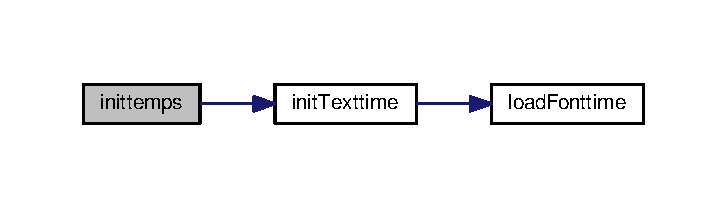
\includegraphics[width=349pt]{utilitaire_8c_a2bbd14a997f1fa7fd246f24ead3b50f8_cgraph}
\end{center}
\end{figure}


\index{utilitaire.\+c@{utilitaire.\+c}!init\+Textscorep1@{init\+Textscorep1}}
\index{init\+Textscorep1@{init\+Textscorep1}!utilitaire.\+c@{utilitaire.\+c}}
\subsubsection[{\texorpdfstring{init\+Textscorep1(\+Text $\ast$\+T)}{initTextscorep1(Text *T)}}]{\setlength{\rightskip}{0pt plus 5cm}int init\+Textscorep1 (
\begin{DoxyParamCaption}
\item[{{\bf Text} $\ast$}]{T}
\end{DoxyParamCaption}
)}\hypertarget{utilitaire_8c_a55245cb1f67d5bd884e547b37bd4d1b3}{}\label{utilitaire_8c_a55245cb1f67d5bd884e547b37bd4d1b3}


To initialize the text T . 


\begin{DoxyParams}{Parameters}
{\em T} & the text \\
\hline
\end{DoxyParams}
\begin{DoxyReturn}{Returns}
int To update score . 
\end{DoxyReturn}

\begin{DoxyParams}{Parameters}
{\em T} & the text of score. \\
\hline
{\em col} & \\
\hline
\end{DoxyParams}
\begin{DoxyReturn}{Returns}
Nothing 
\end{DoxyReturn}


Here is the call graph for this function\+:\nopagebreak
\begin{figure}[H]
\begin{center}
\leavevmode
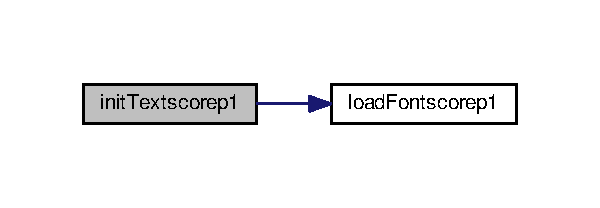
\includegraphics[width=288pt]{utilitaire_8c_a55245cb1f67d5bd884e547b37bd4d1b3_cgraph}
\end{center}
\end{figure}




Here is the caller graph for this function\+:\nopagebreak
\begin{figure}[H]
\begin{center}
\leavevmode
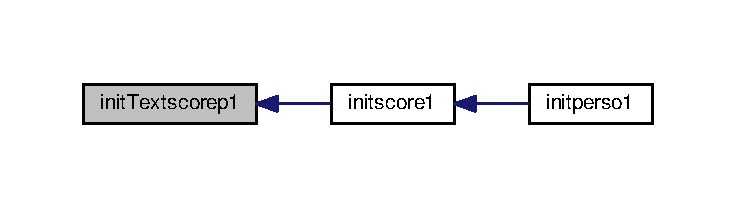
\includegraphics[width=350pt]{utilitaire_8c_a55245cb1f67d5bd884e547b37bd4d1b3_icgraph}
\end{center}
\end{figure}


\index{utilitaire.\+c@{utilitaire.\+c}!init\+Textscorep2@{init\+Textscorep2}}
\index{init\+Textscorep2@{init\+Textscorep2}!utilitaire.\+c@{utilitaire.\+c}}
\subsubsection[{\texorpdfstring{init\+Textscorep2(\+Text $\ast$\+T)}{initTextscorep2(Text *T)}}]{\setlength{\rightskip}{0pt plus 5cm}int init\+Textscorep2 (
\begin{DoxyParamCaption}
\item[{{\bf Text} $\ast$}]{T}
\end{DoxyParamCaption}
)}\hypertarget{utilitaire_8c_a45b667d61b2ed92906aa25efcba9c5a3}{}\label{utilitaire_8c_a45b667d61b2ed92906aa25efcba9c5a3}


To initialize the text T . 


\begin{DoxyParams}{Parameters}
{\em T} & the text \\
\hline
\end{DoxyParams}
\begin{DoxyReturn}{Returns}
int 
\end{DoxyReturn}


Here is the call graph for this function\+:\nopagebreak
\begin{figure}[H]
\begin{center}
\leavevmode
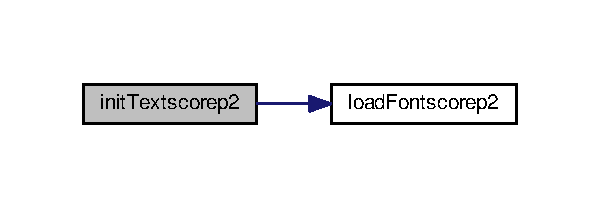
\includegraphics[width=288pt]{utilitaire_8c_a45b667d61b2ed92906aa25efcba9c5a3_cgraph}
\end{center}
\end{figure}




Here is the caller graph for this function\+:\nopagebreak
\begin{figure}[H]
\begin{center}
\leavevmode
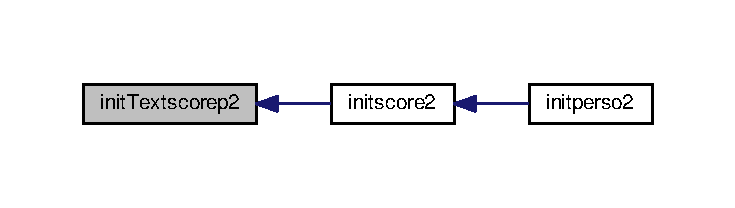
\includegraphics[width=350pt]{utilitaire_8c_a45b667d61b2ed92906aa25efcba9c5a3_icgraph}
\end{center}
\end{figure}


\index{utilitaire.\+c@{utilitaire.\+c}!init\+Texttime@{init\+Texttime}}
\index{init\+Texttime@{init\+Texttime}!utilitaire.\+c@{utilitaire.\+c}}
\subsubsection[{\texorpdfstring{init\+Texttime(\+Text $\ast$\+T)}{initTexttime(Text *T)}}]{\setlength{\rightskip}{0pt plus 5cm}int init\+Texttime (
\begin{DoxyParamCaption}
\item[{{\bf Text} $\ast$}]{T}
\end{DoxyParamCaption}
)}\hypertarget{utilitaire_8c_ae326325c6cbb8e991873fc3da6a8265e}{}\label{utilitaire_8c_ae326325c6cbb8e991873fc3da6a8265e}


To initialize the text T . 


\begin{DoxyParams}{Parameters}
{\em T} & the text \\
\hline
\end{DoxyParams}
\begin{DoxyReturn}{Returns}
int 
\end{DoxyReturn}


Here is the call graph for this function\+:\nopagebreak
\begin{figure}[H]
\begin{center}
\leavevmode
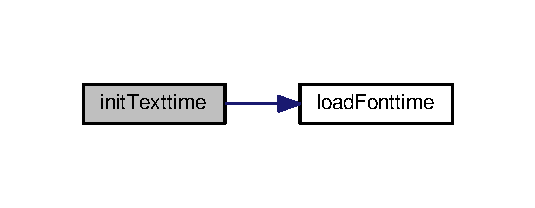
\includegraphics[width=257pt]{utilitaire_8c_ae326325c6cbb8e991873fc3da6a8265e_cgraph}
\end{center}
\end{figure}




Here is the caller graph for this function\+:\nopagebreak
\begin{figure}[H]
\begin{center}
\leavevmode
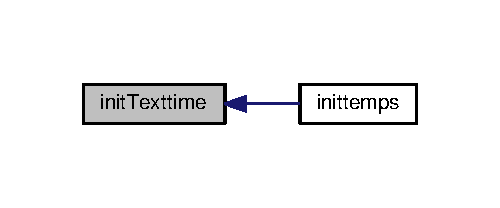
\includegraphics[width=240pt]{utilitaire_8c_ae326325c6cbb8e991873fc3da6a8265e_icgraph}
\end{center}
\end{figure}


\index{utilitaire.\+c@{utilitaire.\+c}!init\+Textviep1@{init\+Textviep1}}
\index{init\+Textviep1@{init\+Textviep1}!utilitaire.\+c@{utilitaire.\+c}}
\subsubsection[{\texorpdfstring{init\+Textviep1(\+Text $\ast$\+T)}{initTextviep1(Text *T)}}]{\setlength{\rightskip}{0pt plus 5cm}int init\+Textviep1 (
\begin{DoxyParamCaption}
\item[{{\bf Text} $\ast$}]{T}
\end{DoxyParamCaption}
)}\hypertarget{utilitaire_8c_a9f0f8886c9c3e6e8469cb1a24a8c9ed6}{}\label{utilitaire_8c_a9f0f8886c9c3e6e8469cb1a24a8c9ed6}


To initialize the text T . 


\begin{DoxyParams}{Parameters}
{\em T} & the text \\
\hline
\end{DoxyParams}
\begin{DoxyReturn}{Returns}
int 
\end{DoxyReturn}


Here is the call graph for this function\+:\nopagebreak
\begin{figure}[H]
\begin{center}
\leavevmode
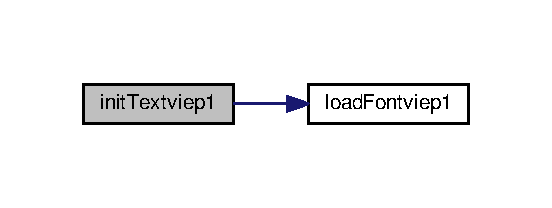
\includegraphics[width=265pt]{utilitaire_8c_a9f0f8886c9c3e6e8469cb1a24a8c9ed6_cgraph}
\end{center}
\end{figure}




Here is the caller graph for this function\+:\nopagebreak
\begin{figure}[H]
\begin{center}
\leavevmode
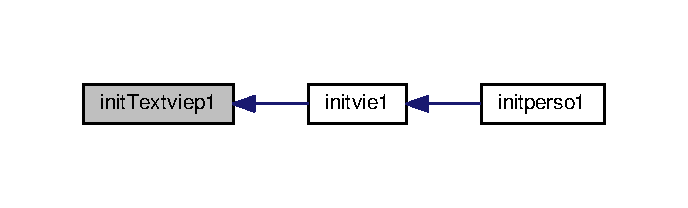
\includegraphics[width=330pt]{utilitaire_8c_a9f0f8886c9c3e6e8469cb1a24a8c9ed6_icgraph}
\end{center}
\end{figure}


\index{utilitaire.\+c@{utilitaire.\+c}!init\+Textviep2@{init\+Textviep2}}
\index{init\+Textviep2@{init\+Textviep2}!utilitaire.\+c@{utilitaire.\+c}}
\subsubsection[{\texorpdfstring{init\+Textviep2(\+Text $\ast$\+T)}{initTextviep2(Text *T)}}]{\setlength{\rightskip}{0pt plus 5cm}int init\+Textviep2 (
\begin{DoxyParamCaption}
\item[{{\bf Text} $\ast$}]{T}
\end{DoxyParamCaption}
)}\hypertarget{utilitaire_8c_ad140cfd864e9a32a4209627b2c4388dd}{}\label{utilitaire_8c_ad140cfd864e9a32a4209627b2c4388dd}


To initialize the text T . 


\begin{DoxyParams}{Parameters}
{\em T} & the text \\
\hline
\end{DoxyParams}
\begin{DoxyReturn}{Returns}
int 
\end{DoxyReturn}


Here is the call graph for this function\+:\nopagebreak
\begin{figure}[H]
\begin{center}
\leavevmode
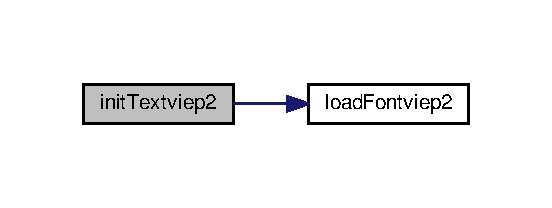
\includegraphics[width=265pt]{utilitaire_8c_ad140cfd864e9a32a4209627b2c4388dd_cgraph}
\end{center}
\end{figure}




Here is the caller graph for this function\+:\nopagebreak
\begin{figure}[H]
\begin{center}
\leavevmode
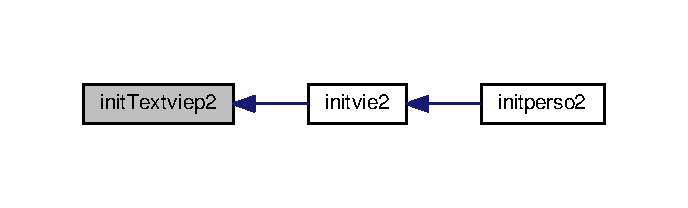
\includegraphics[width=330pt]{utilitaire_8c_ad140cfd864e9a32a4209627b2c4388dd_icgraph}
\end{center}
\end{figure}


\index{utilitaire.\+c@{utilitaire.\+c}!load\+Fontscorep1@{load\+Fontscorep1}}
\index{load\+Fontscorep1@{load\+Fontscorep1}!utilitaire.\+c@{utilitaire.\+c}}
\subsubsection[{\texorpdfstring{load\+Fontscorep1(\+Text $\ast$\+T, char $\ast$path)}{loadFontscorep1(Text *T, char *path)}}]{\setlength{\rightskip}{0pt plus 5cm}int load\+Fontscorep1 (
\begin{DoxyParamCaption}
\item[{{\bf Text} $\ast$}]{T, }
\item[{char $\ast$}]{path}
\end{DoxyParamCaption}
)}\hypertarget{utilitaire_8c_a51c7c5c649ffa053546af592ad26fe9b}{}\label{utilitaire_8c_a51c7c5c649ffa053546af592ad26fe9b}


To load the font T . 


\begin{DoxyParams}{Parameters}
{\em T} & the text \\
\hline
{\em path} & the font \\
\hline
\end{DoxyParams}
\begin{DoxyReturn}{Returns}
int 
\end{DoxyReturn}


Here is the caller graph for this function\+:\nopagebreak
\begin{figure}[H]
\begin{center}
\leavevmode
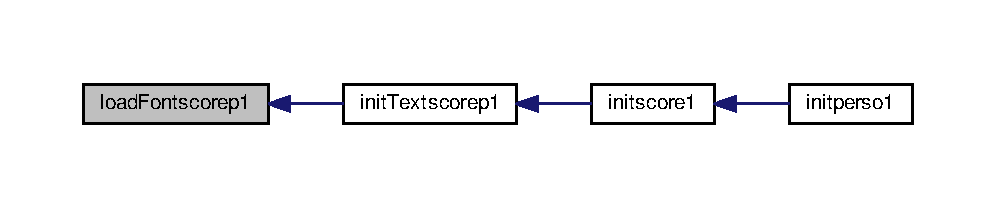
\includegraphics[width=350pt]{utilitaire_8c_a51c7c5c649ffa053546af592ad26fe9b_icgraph}
\end{center}
\end{figure}


\index{utilitaire.\+c@{utilitaire.\+c}!load\+Fontscorep2@{load\+Fontscorep2}}
\index{load\+Fontscorep2@{load\+Fontscorep2}!utilitaire.\+c@{utilitaire.\+c}}
\subsubsection[{\texorpdfstring{load\+Fontscorep2(\+Text $\ast$\+T, char $\ast$path)}{loadFontscorep2(Text *T, char *path)}}]{\setlength{\rightskip}{0pt plus 5cm}int load\+Fontscorep2 (
\begin{DoxyParamCaption}
\item[{{\bf Text} $\ast$}]{T, }
\item[{char $\ast$}]{path}
\end{DoxyParamCaption}
)}\hypertarget{utilitaire_8c_a47f18f3dfebbf72ac94e1ab431f2212b}{}\label{utilitaire_8c_a47f18f3dfebbf72ac94e1ab431f2212b}


To load the font T . 


\begin{DoxyParams}{Parameters}
{\em T} & the text \\
\hline
{\em path} & the font \\
\hline
\end{DoxyParams}
\begin{DoxyReturn}{Returns}
int 
\end{DoxyReturn}


Here is the caller graph for this function\+:\nopagebreak
\begin{figure}[H]
\begin{center}
\leavevmode
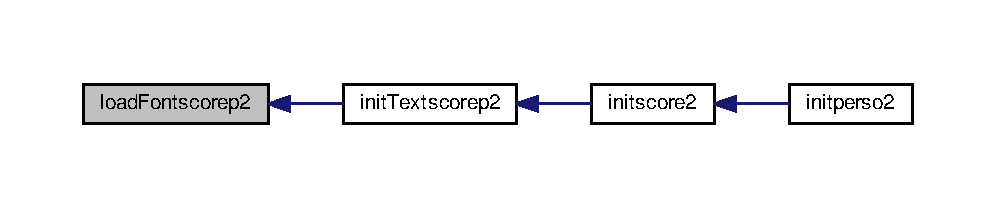
\includegraphics[width=350pt]{utilitaire_8c_a47f18f3dfebbf72ac94e1ab431f2212b_icgraph}
\end{center}
\end{figure}


\index{utilitaire.\+c@{utilitaire.\+c}!load\+Fonttime@{load\+Fonttime}}
\index{load\+Fonttime@{load\+Fonttime}!utilitaire.\+c@{utilitaire.\+c}}
\subsubsection[{\texorpdfstring{load\+Fonttime(\+Text $\ast$\+T, char $\ast$path)}{loadFonttime(Text *T, char *path)}}]{\setlength{\rightskip}{0pt plus 5cm}int load\+Fonttime (
\begin{DoxyParamCaption}
\item[{{\bf Text} $\ast$}]{T, }
\item[{char $\ast$}]{path}
\end{DoxyParamCaption}
)}\hypertarget{utilitaire_8c_abf80670169d96288d8a4b673ad90a80a}{}\label{utilitaire_8c_abf80670169d96288d8a4b673ad90a80a}


To load the font T . 


\begin{DoxyParams}{Parameters}
{\em T} & the text \\
\hline
{\em path} & the font \\
\hline
\end{DoxyParams}
\begin{DoxyReturn}{Returns}
int 
\end{DoxyReturn}


Here is the caller graph for this function\+:\nopagebreak
\begin{figure}[H]
\begin{center}
\leavevmode
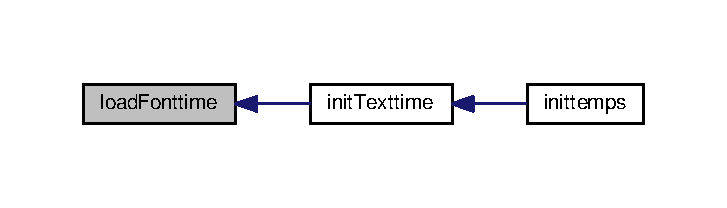
\includegraphics[width=349pt]{utilitaire_8c_abf80670169d96288d8a4b673ad90a80a_icgraph}
\end{center}
\end{figure}


\index{utilitaire.\+c@{utilitaire.\+c}!load\+Fontviep1@{load\+Fontviep1}}
\index{load\+Fontviep1@{load\+Fontviep1}!utilitaire.\+c@{utilitaire.\+c}}
\subsubsection[{\texorpdfstring{load\+Fontviep1(\+Text $\ast$\+T, char $\ast$path)}{loadFontviep1(Text *T, char *path)}}]{\setlength{\rightskip}{0pt plus 5cm}int load\+Fontviep1 (
\begin{DoxyParamCaption}
\item[{{\bf Text} $\ast$}]{T, }
\item[{char $\ast$}]{path}
\end{DoxyParamCaption}
)}\hypertarget{utilitaire_8c_aa94706beac591b2437d6e27e8b1a6551}{}\label{utilitaire_8c_aa94706beac591b2437d6e27e8b1a6551}


To load the font T . 


\begin{DoxyParams}{Parameters}
{\em T} & the text \\
\hline
{\em path} & the font \\
\hline
\end{DoxyParams}
\begin{DoxyReturn}{Returns}
int 
\end{DoxyReturn}


Here is the caller graph for this function\+:\nopagebreak
\begin{figure}[H]
\begin{center}
\leavevmode
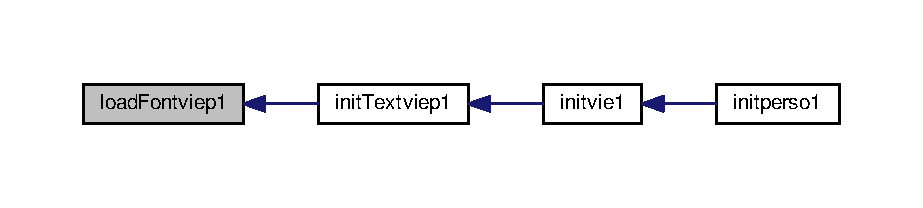
\includegraphics[width=350pt]{utilitaire_8c_aa94706beac591b2437d6e27e8b1a6551_icgraph}
\end{center}
\end{figure}


\index{utilitaire.\+c@{utilitaire.\+c}!load\+Fontviep2@{load\+Fontviep2}}
\index{load\+Fontviep2@{load\+Fontviep2}!utilitaire.\+c@{utilitaire.\+c}}
\subsubsection[{\texorpdfstring{load\+Fontviep2(\+Text $\ast$\+T, char $\ast$path)}{loadFontviep2(Text *T, char *path)}}]{\setlength{\rightskip}{0pt plus 5cm}int load\+Fontviep2 (
\begin{DoxyParamCaption}
\item[{{\bf Text} $\ast$}]{T, }
\item[{char $\ast$}]{path}
\end{DoxyParamCaption}
)}\hypertarget{utilitaire_8c_a14b318435a12ec6e651f120e034993fe}{}\label{utilitaire_8c_a14b318435a12ec6e651f120e034993fe}


To load the font T . 


\begin{DoxyParams}{Parameters}
{\em T} & the text \\
\hline
{\em path} & the font \\
\hline
\end{DoxyParams}
\begin{DoxyReturn}{Returns}
int 
\end{DoxyReturn}


Here is the caller graph for this function\+:\nopagebreak
\begin{figure}[H]
\begin{center}
\leavevmode
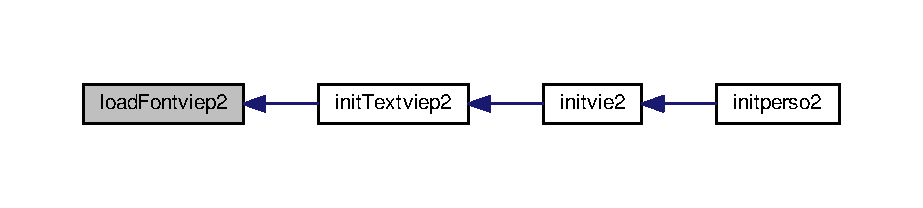
\includegraphics[width=350pt]{utilitaire_8c_a14b318435a12ec6e651f120e034993fe_icgraph}
\end{center}
\end{figure}


\index{utilitaire.\+c@{utilitaire.\+c}!Timer@{Timer}}
\index{Timer@{Timer}!utilitaire.\+c@{utilitaire.\+c}}
\subsubsection[{\texorpdfstring{Timer(int $\ast$tempsdebut)}{Timer(int *tempsdebut)}}]{\setlength{\rightskip}{0pt plus 5cm}void Timer (
\begin{DoxyParamCaption}
\item[{int $\ast$}]{tempsdebut}
\end{DoxyParamCaption}
)}\hypertarget{utilitaire_8c_a5929c26a66049460dc58b8c92a6d0b2f}{}\label{utilitaire_8c_a5929c26a66049460dc58b8c92a6d0b2f}


To count \hyperlink{structTime}{Time} . 


\begin{DoxyParams}{Parameters}
{\em tempsdebut} & \\
\hline
\end{DoxyParams}
\begin{DoxyReturn}{Returns}
nothing 
\end{DoxyReturn}


Here is the caller graph for this function\+:\nopagebreak
\begin{figure}[H]
\begin{center}
\leavevmode
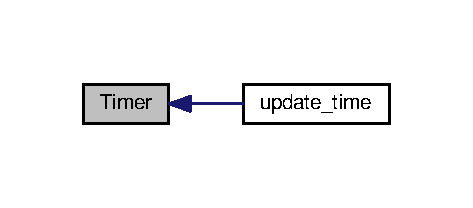
\includegraphics[width=227pt]{utilitaire_8c_a5929c26a66049460dc58b8c92a6d0b2f_icgraph}
\end{center}
\end{figure}


\index{utilitaire.\+c@{utilitaire.\+c}!update\+\_\+scorep1@{update\+\_\+scorep1}}
\index{update\+\_\+scorep1@{update\+\_\+scorep1}!utilitaire.\+c@{utilitaire.\+c}}
\subsubsection[{\texorpdfstring{update\+\_\+scorep1(\+Text $\ast$\+T, int $\ast$score, collision col)}{update_scorep1(Text *T, int *score, collision col)}}]{\setlength{\rightskip}{0pt plus 5cm}void update\+\_\+scorep1 (
\begin{DoxyParamCaption}
\item[{{\bf Text} $\ast$}]{T, }
\item[{int $\ast$}]{score, }
\item[{{\bf collision}}]{col}
\end{DoxyParamCaption}
)}\hypertarget{utilitaire_8c_a43d377ba6c658485c2058b8c4feafc45}{}\label{utilitaire_8c_a43d377ba6c658485c2058b8c4feafc45}


To update score . 


\begin{DoxyParams}{Parameters}
{\em T} & the text of score. \\
\hline
{\em col} & \\
\hline
\end{DoxyParams}
\begin{DoxyReturn}{Returns}
Nothing 
\end{DoxyReturn}


Here is the caller graph for this function\+:\nopagebreak
\begin{figure}[H]
\begin{center}
\leavevmode
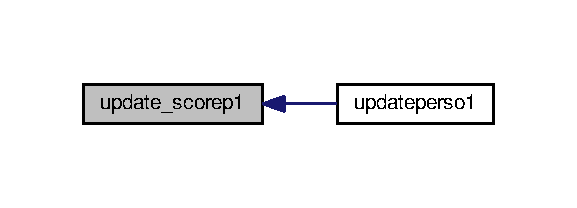
\includegraphics[width=277pt]{utilitaire_8c_a43d377ba6c658485c2058b8c4feafc45_icgraph}
\end{center}
\end{figure}


\index{utilitaire.\+c@{utilitaire.\+c}!update\+\_\+scorep2@{update\+\_\+scorep2}}
\index{update\+\_\+scorep2@{update\+\_\+scorep2}!utilitaire.\+c@{utilitaire.\+c}}
\subsubsection[{\texorpdfstring{update\+\_\+scorep2(\+Text $\ast$\+T, int $\ast$score, collision col)}{update_scorep2(Text *T, int *score, collision col)}}]{\setlength{\rightskip}{0pt plus 5cm}void update\+\_\+scorep2 (
\begin{DoxyParamCaption}
\item[{{\bf Text} $\ast$}]{T, }
\item[{int $\ast$}]{score, }
\item[{{\bf collision}}]{col}
\end{DoxyParamCaption}
)}\hypertarget{utilitaire_8c_ad8da31bfa2e50fc4e771bfad1d769c95}{}\label{utilitaire_8c_ad8da31bfa2e50fc4e771bfad1d769c95}


To update score . 


\begin{DoxyParams}{Parameters}
{\em T} & the text of score. \\
\hline
{\em col} & \\
\hline
\end{DoxyParams}
\begin{DoxyReturn}{Returns}
Nothing 
\end{DoxyReturn}


Here is the caller graph for this function\+:\nopagebreak
\begin{figure}[H]
\begin{center}
\leavevmode
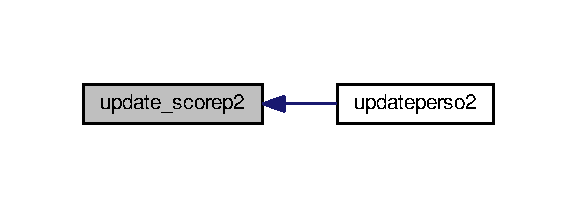
\includegraphics[width=277pt]{utilitaire_8c_ad8da31bfa2e50fc4e771bfad1d769c95_icgraph}
\end{center}
\end{figure}


\index{utilitaire.\+c@{utilitaire.\+c}!update\+\_\+time@{update\+\_\+time}}
\index{update\+\_\+time@{update\+\_\+time}!utilitaire.\+c@{utilitaire.\+c}}
\subsubsection[{\texorpdfstring{update\+\_\+time(\+Time $\ast$\+T)}{update_time(Time *T)}}]{\setlength{\rightskip}{0pt plus 5cm}void update\+\_\+time (
\begin{DoxyParamCaption}
\item[{{\bf Time} $\ast$}]{T}
\end{DoxyParamCaption}
)}\hypertarget{utilitaire_8c_abc558b87e2e48a9f354536407ee6abbd}{}\label{utilitaire_8c_abc558b87e2e48a9f354536407ee6abbd}


To update time . 


\begin{DoxyParams}{Parameters}
{\em T} & the text of time. \\
\hline
\end{DoxyParams}
\begin{DoxyReturn}{Returns}
Nothing 
\end{DoxyReturn}


Here is the call graph for this function\+:\nopagebreak
\begin{figure}[H]
\begin{center}
\leavevmode
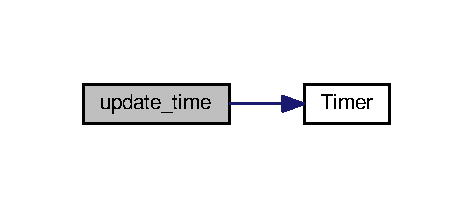
\includegraphics[width=227pt]{utilitaire_8c_abc558b87e2e48a9f354536407ee6abbd_cgraph}
\end{center}
\end{figure}


\index{utilitaire.\+c@{utilitaire.\+c}!update\+\_\+viep1@{update\+\_\+viep1}}
\index{update\+\_\+viep1@{update\+\_\+viep1}!utilitaire.\+c@{utilitaire.\+c}}
\subsubsection[{\texorpdfstring{update\+\_\+viep1(\+Text $\ast$\+T, int $\ast$vies, collision col)}{update_viep1(Text *T, int *vies, collision col)}}]{\setlength{\rightskip}{0pt plus 5cm}void update\+\_\+viep1 (
\begin{DoxyParamCaption}
\item[{{\bf Text} $\ast$}]{T, }
\item[{int $\ast$}]{vies, }
\item[{{\bf collision}}]{col}
\end{DoxyParamCaption}
)}\hypertarget{utilitaire_8c_a8876655d6513fd06f7c4a3d07f7d92e3}{}\label{utilitaire_8c_a8876655d6513fd06f7c4a3d07f7d92e3}


To update vie . 


\begin{DoxyParams}{Parameters}
{\em T} & the text of vie. \\
\hline
{\em vie} & nomber of life. \\
\hline
{\em col} & . \\
\hline
\end{DoxyParams}
\begin{DoxyReturn}{Returns}
Nothing 
\end{DoxyReturn}


Here is the caller graph for this function\+:\nopagebreak
\begin{figure}[H]
\begin{center}
\leavevmode
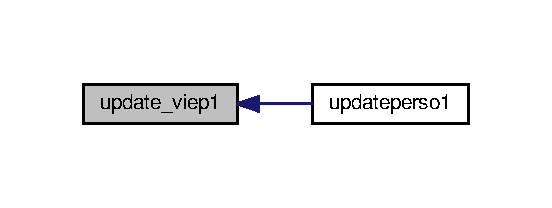
\includegraphics[width=265pt]{utilitaire_8c_a8876655d6513fd06f7c4a3d07f7d92e3_icgraph}
\end{center}
\end{figure}


\index{utilitaire.\+c@{utilitaire.\+c}!update\+\_\+viep2@{update\+\_\+viep2}}
\index{update\+\_\+viep2@{update\+\_\+viep2}!utilitaire.\+c@{utilitaire.\+c}}
\subsubsection[{\texorpdfstring{update\+\_\+viep2(\+Text $\ast$\+T, int $\ast$vies, collision col)}{update_viep2(Text *T, int *vies, collision col)}}]{\setlength{\rightskip}{0pt plus 5cm}void update\+\_\+viep2 (
\begin{DoxyParamCaption}
\item[{{\bf Text} $\ast$}]{T, }
\item[{int $\ast$}]{vies, }
\item[{{\bf collision}}]{col}
\end{DoxyParamCaption}
)}\hypertarget{utilitaire_8c_a9601e16efa9686e1f560ef5a4a4727bf}{}\label{utilitaire_8c_a9601e16efa9686e1f560ef5a4a4727bf}


To update vie . 


\begin{DoxyParams}{Parameters}
{\em T} & the text of vie. \\
\hline
{\em vie} & nomber of life. \\
\hline
{\em col} & . \\
\hline
\end{DoxyParams}
\begin{DoxyReturn}{Returns}
Nothing 
\end{DoxyReturn}


Here is the caller graph for this function\+:\nopagebreak
\begin{figure}[H]
\begin{center}
\leavevmode
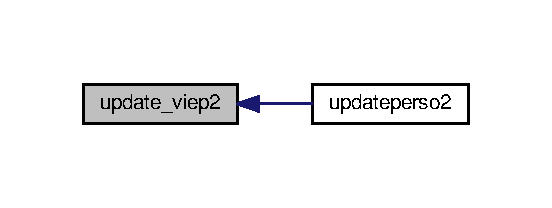
\includegraphics[width=265pt]{utilitaire_8c_a9601e16efa9686e1f560ef5a4a4727bf_icgraph}
\end{center}
\end{figure}



%--- End generated contents ---

% Index
\backmatter
\newpage
\phantomsection
\clearemptydoublepage
\addcontentsline{toc}{chapter}{Index}
\printindex

\end{document}
